
% This is "sig-alternate.tex" V2.0 May 2012
% This file should be compiled with V2.5 of "sig-alternate.cls" May 2012
%
% This example file demonstrates the use of the 'sig-alternate.cls'
% V2.5 LaTeX2e document class file. It is for those submitting
% articles to ACM Conference Proceedings WHO DO NOT WISH TO
% STRICTLY ADHERE TO THE SIGS (PUBS-BOARD-ENDORSED) STYLE.
% The 'sig-alternate.cls' file will produce a similar-looking,
% albeit, 'tighter' paper resulting in, invariably, fewer pages.
%
% ----------------------------------------------------------------------------------------------------------------
% This .tex file (and associated .cls V2.5) produces:
%       1) The Permission Statement
%       2) The Conference (location) Info information
%       3) The Copyright Line with ACM data
%       4) NO page numbers
%
% as against the acm_proc_article-sp.cls file which
% DOES NOT produce 1) thru' 3) above.
%
% Using 'sig-alternate.cls' you have control, however, from within
% the source .tex file, over both the CopyrightYear
% (defaulted to 200X) and the ACM Copyright Data
% (defaulted to X-XXXXX-XX-X/XX/XX).
% e.g.
% \CopyrightYear{2007} will cause 2007 to appear in the copyright line.
% \crdata{0-12345-67-8/90/12} will cause 0-12345-67-8/90/12 to appear in the copyright line.
%
% ---------------------------------------------------------------------------------------------------------------
% This .tex source is an example which *does* use
% the .bib file (from which the .bbl file % is produced).
% REMEMBER HOWEVER: After having produced the .bbl file,
% and prior to final submission, you *NEED* to 'insert'
% your .bbl file into your source .tex file so as to provide
% ONE 'self-contained' source file.
%
% ================= IF YOU HAVE QUESTIONS =======================
% Questions regarding the SIGS styles, SIGS policies and
% procedures, Conferences etc. should be sent to
% Adrienne Griscti (griscti@acm.org)
%
% Technical questions _only_ to
% Gerald Murray (murray@hq.acm.org)
% ===============================================================
%
% For tracking purposes - this is V2.0 - May 2012

\documentclass{sig-alternate}

\usepackage{cite}
\usepackage{float}

\usepackage{setspace}
\usepackage{multirow}
\usepackage{array}
\usepackage{import}
\usepackage{tikz}
\usepackage[bookmarks=false]{hyperref}
\usepackage[hyphenbreaks]{breakurl}
\usepackage{graphicx}
\usepackage{xcolor,colortbl}
\usepackage{tabularx}
\usepackage{flushend}
\usepackage{amsmath}
\usepackage{subcaption}

\begin{document}
%
% --- Author Metadata here ---
\conferenceinfo{WWW}{'16 Montereal, Canada}
%\CopyrightYear{2007} % Allows default copyright year (20XX) to be over-ridden - IF NEED BE.
%\crdata{0-12345-67-8/90/01}  % Allows default copyright data (0-89791-88-6/97/05) to be over-ridden - IF NEED BE.
% --- End of Author Metadata ---

\title{Adoption and evolution of social networks from a cohort perspective}

%\title{Alternate {\ttlit ACM} SIG Proceedings Paper in LaTeX
%Format\titlenote{(Produces the permission block, and
%copyright information). For use with
%SIG-ALTERNATE.CLS. Supported by ACM.}}
%\subtitle{[Extended Abstract]
%\titlenote{A full version of this paper is available as
%\textit{Author's Guide to Preparing ACM SIG Proceedings Using
%\LaTeX$2_\epsilon$\ and BibTeX} at
%\texttt{www.acm.org/eaddress.htm}}}
%
% You need the command \numberofauthors to handle the 'placement
% and alignment' of the authors beneath the title.
%
% For aesthetic reasons, we recommend 'three authors at a time'
% i.e. three 'name/affiliation blocks' be placed beneath the title.
%
% NOTE: You are NOT restricted in how many 'rows' of
% "name/affiliations" may appear. We just ask that you restrict
% the number of 'columns' to three.
%
% Because of the available 'opening page real-estate'
% we ask you to refrain from putting more than six authors
% (two rows with three columns) beneath the article title.
% More than six makes the first-page appear very cluttered indeed.
%
% Use the \alignauthor commands to handle the names
% and affiliations for an 'aesthetic maximum' of six authors.
% Add names, affiliations, addresses for
% the seventh etc. author(s) as the argument for the
% \additionalauthors command.
% These 'additional authors' will be output/set for you
% without further effort on your part as the last section in
% the body of your article BEFORE References or any Appendices.

\numberofauthors{4} %  in this sample file, there are a *total*
% of EIGHT authors. SIX appear on the 'first-page' (for formatting
% reasons) and the remaining two appear in the \additionalauthors section.
%
\author{
% You can go ahead and credit any number of authors here,
% e.g. one 'row of three' or two rows (consisting of one row of three
% and a second row of one, two or three).
%
% The command \alignauthor (no curly braces needed) should
% precede each author name, affiliation/snail-mail address and
% e-mail address. Additionally, tag each line of
% affiliation/address with \affaddr, and tag the
% e-mail address with \email.
%
% 1st. author
\alignauthor
Samuel Barbosa\\
       \affaddr{Institute of Mathematics and Statistics}\\
       \affaddr{University of S\~ao Paulo}\\
       \affaddr{S\~ao Paulo, Brazil}\\
       \email{sam@ime.usp.br}
 %2nd. author
\alignauthor
Dan Cosley\\
       \affaddr{Department of Information Science}\\
       \affaddr{Cornell University}\\
       \affaddr{Ithaca, NY 14853 USA}\\
       \email{danco@cs.cornell.edu}
 %3rd. author
\alignauthor
Amit Sharma\\
       \affaddr{Microsoft Research}\\
       \affaddr{New York, NY 10011 USA}\\
       \email{amshar@microsoft.com}
 %4th. author
\and
\alignauthor
Roberto M. Cesar-Jr\\
       \affaddr{Institute of Mathematics and Statistics}\\
       \affaddr{University of S\~ao Paulo}\\
       \affaddr{S\~ao Paulo, Brazil}\\
       \email{cesar@ime.usp.br}
}
% There's nothing stopping you putting the seventh, eighth, etc.
% author on the opening page (as the 'third row') but we ask,
% for aesthetic reasons that you place these 'additional authors'
% in the \additional authors block, viz.
%\additionalauthors{Additional authors: John Smith (The Th{\o}rv{\"a}ld Group,
%email: {\texttt{jsmith@affiliation.org}}) and Julius P.~Kumquat
%(The Kumquat Consortium, email: {\texttt{jpkumquat@consortium.net}}).}

\date{10 October 2015}
% Just remember to make sure that the TOTAL number of authors
% is the number that will appear on the first page PLUS the
% number that will appear in the \additionalauthors section.

\maketitle
\begin{abstract}
Online communities provide a fertile ground for analyzing people's behavior and improving our understanding of social processes. However, like any complex social system, the key part is detail in identifying and accounting for underlying heterogeneity and selection effects among people in these communities. Using Reddit as an example community, we study the evolution of users based on comments and submissions data from 2007 to 2014, creating a cohort of users who join each year. Even with one of the simplest sources of differentiation between users---their age in the community---we find wide differences in people's behavior, including comment activity, effort and survival, both within cohorts and with the averages over the whole community. Not controlling for these variations may not only dilute the overall effects that we observe, but in some cases, it can lead us to the wrong conclusions (Simpson's paradox).  These observations can be puzzling: for instance, we observe that average comment length decreases over any fixed period of time, but comment length in each cohort of users steadily increases during the same period after an abrupt initial drop. Finally, we analyze subcommunities on Reddit through the same lens of age and we find an enormous first-mover advantage: subreddits created early in the community's history are orders of magnitude more active than even successful subreddits created later, even among cohorts of users who join much later.
\end{abstract}

\keywords{user behavior;cohort;reddit}

% A category with the (minimum) three required fields
%\category{H.4}{Information Systems Applications}{Miscellaneous}
%A category including the fourth, optional field follows...
%\category{D.2.8}{Software Engineering}{Metrics}[complexity measures, performance measures]
%\terms{Theory}
%\keywords{ACM proceedings, \LaTeX, text tagging}


\section{Introduction}

Understanding the evolution of users in a social network is essential for a variety of tasks: monitoring community health, predicting individual user trajectories, and supporting effective recommendations, among others.  Many works aim at explaining these temporal aspects of evolution. Some adopt a point of view of the whole network and try to understand more general patterns of behavior \cite{Zhu2014, Kooti2010}, while others adopt a more user-centric point of view and try to model \cite{Correa2010, Priedhorsky2007, Panciera2009, Welser2011} or predict \cite{Danescu-niculescu-mizil2013} individuals' behavior.

These approaches often combine all available data into aggregate analyses of the entire community over its entire history.  This can be a natural response to limitations in the amount of available data: many datasets capture a small part of the community's history \cite{Artzi2012}; timestamps may not be available \cite{Priedhorsky2007, Pujol2010}; snapshots may provide limited views of the community \cite{Cosley2010}; or the community itself might be small \cite{Lewis2008}.  Aggregate time-based analysis are also a natural first way to address questions of community evolution.

However, we argue it is likely that many of these aggregated views are misleading. The conditions under which users join the community may vary greatly over time, and this might impact their behavior \cite{Miller2015}.  Among other things, the popularity, purpose, features, interface, and algorithms can change: Wikipedia circa 2005 and circa 2015 are very different, as are Facebook of 2005 and 2015.  Analysis---including some of our own past work---that fail to account for this change may miss important details of what is really going on.

We support this argument through an analysis of user effort in Reddit, one of the most popular and long-running online communities, based on a very large, recently released dataset of posting behavior.  We address a number of questions commonly raised about users' effort in online communities: how active are users, how hard do they work, and what kinds of things do they do?  In each case, we compare aggregate analyses of posting behavior to ones that treat users in Reddit as yearly cohorts, and views that focus on calendar time versus user-referential views that normalize behavior based on the creation date of a user.  We also look at differences within yearly cohorts, seeking differences between shorter and longer-lived users.

We find that even simple accountings for time reveal additional insights about Reddit beyond what commonly performed aggregate analyses can provide.  Users who join Reddit earlier post more and longer comments than those who join later, while users who survive longer start out both more active and more likely to comment than submit compared to users who leave Reddit early; none of these findings are obvious from commonly used analysis of user behavior.  

Further, we find that aggregate analysis can be downright misleading.  For instance, although average comment length decreases over time in an aggregate view, the comment length for surviving users increases over time in every cohort.  Likewise, an aggregate analysis suggests that longer-lived users post more over time; this is not the case.  Instead, users come into Reddit as active as they will ever be (somewhat akin to Panciera et al.'s finding that Wikipedians are ``born, not made'' \cite{Panciera2009}), and the rise in average activity for surviving users over time is driven fully by lower-activity users leaving early.     

We see this paper as both making specific contributions to understanding behavior in Reddit and a more general contribution around the importance of considering change over time in analyzing online communities. 

%%Amit: write about concrete contributions? Not sure.
%% DC 15: I tried to put some of that into the "we find" para above.

%% DC 12: I think we should narrow the story and focus it on user effort.  We can define things like the joint subreddit/user cohort analysis as a kind of effort question, but we need to have a story that's narrow enough to tell in a believable way and that people can hang their hats on.  That's what I tried to do here.

%% DC 12: I like the _idea_ here of trying to explain why we see this kind of aggregate analysis.  This execution doesn't work so well for me, though.  It's not clear why a small community over the years, or snapshots, or pulled data are the reason people don't do analyses.  But, it did cause me to write the 
%In doing these analyses, it is quite common for researchers to have limited data in terms of time---one, or a few snapshots of the network are available\cite{}---or in terms of scope---only a small community is observed over the years \cite{Lewis2008}.
%% DC 12: This doesn't really help tell the story.
%It is also not unheard of cases in which datasets were made unavailable upon request from these social networks \footnote{\url{http://twitter.mpi-sws.org/}}.
%These increase the difficulty of scaling temporal models and limit the networks on which is possible to perform these kind of analysis --- Wikipedia is known for having their whole data available \cite{Panciera2009, Priedhorsky2007}. 

%% DC 12: Cites probably want to be put in here as they are found. 
\section{Previous Work}

\begin{itemize}
    \item The Taste for Privacy: An Analysis of College Student Privacy Settings in an Online Social Network \cite{Lewis2008}: Studies which characteristics are predictive of whether or not users are going to set their profile as public or private in Facebook. Raises questions about the limitations of the work because data collected came from a single cohort of users in a college.

    \item Social selection and peer influence in an online social network \cite{Lewis2012a}: Yet another study based on a single cohort of Facebook data for college students. Discuss the relationship between homophily in creating connections and influence over the course of a connection.

    \item Who interacts on the Web?: The intersection of users' personality and social media use \cite{Correa2010}: Studies how personality traits correlate with social media usage controlling for demographic variables age, gender, race, education and income. One of the research questions was whether user age cohorts influence social media usage. They found significant correlation of some personality traits with social media usage for the younger cohort (users from 18 to 29). They also acknowledge the lack of research on how age influences interaction on social media, pointing out that significant differences emerge from people that grew on a digital environment when compared to the ones that were introduced to the technology at a later time.

    \item ``I LOVE THIS SITE!'' vs. ``It's a little girly'': Perceptions of and Initial User Experience with Pinterest \cite{Miller2015}: Initial experience matters! 

    \item No Country for Old Members : User Lifecycle and Linguistic Change in Online Communities \cite{Danescu-niculescu-mizil2013}: User experience changes their behavior over time but they also come with some linguistic predispositions.

    \item All Who Wander : On the Prevalence and Characteristics of Multi-community Engagement \cite{Tan2015}: Survival does depend on user initial activities.

    \item Wikipedians are Born, Not Made \cite{Panciera2009}: Users do have predispositions. Does that mean they do not change and we are simply sampling differently?

    \item Creating , Destroying , and Restoring Value in Wikipedia \cite{Priedhorsky2007}: Not clear where it fits.

    \item The Impact of Membership Overlap on the Survival of Online Communities \cite{Zhu2014}: The survival of communities depends on the type of users that participate in it, and sharing certain types of users --- core members from other communities that are not core members in the focal community --- can be beneficial for community survival. Also, concepts of young and mature communities play a important role when analyzing community activity level, where young communities benefit from sharing members from matures communities. 

    \item No Country for Old Members : User Lifecycle and Linguistic Change in Online Communities: Highlights the interplay on community language change and user adoption of new norms. As a general pattern, newcomers start learning the norms of the community and, as they age, they become more conservative in adopting new norms. Users that are more flexible in assimilating new norms have a higher survival rate.
    
\end{itemize}
\section{Data: Reddit as a community}

%% DC 14: Moving this to the end of prev work to give a little more context and beef; things felt redundant between that and this and it feels better there.

\subsection{What is Reddit, briefly}

%% Sam 11: Improving the caption
\begin{figure}[!tb]
\centering

\includegraphics[width=0.45\textwidth,natwidth=964,natheight=823]{./images/reddit.png}
\caption{Reddit interface when visualizing a submission. This is Patrick Stewart's ``AmA'' (ask me anything) in ``IAmA'' (I am a), a submission where he answers users' questions in the comments. We can see the most upvoted comment and Patrick's answer right below.}
\label{fig:reddit}
\end{figure}

Reddit is one of the largest sharing and discussion communities on the Web.  According to Alexa, as of late 2015 Reddit is in the top 15 sites in the U.S. and the top 35 in the world in terms of monthly unique visitors.  It consists of a large number of subreddits (853,000 as of June 21st, 2015\footnote{\cite{RedditStatistics} provides more statistics about Reddit.}), each of which focuses on a particular purpose.  Many subreddits are primarily about sharing web content from other sites: in ``Pics'', ``News'', ``Funny'', ``Gaming'', and many other communities, users (``Redditors'') make ``submissions'' of links posted at other sites that they think are interesting.  In other subreddits, Redditors primarily write text-based ``self-posts'': ``AskReddit'', ``IAmA'', and ``ShowerThoughts'' are places where people can ask questions and share stories of their own lives.  Generically, we will refer to submissions and text posts as ``submissions''.  

Each submission can be imagined as the root of a threaded comment tree, in which Redditors can comment on submissions or each other's comments.  Redditors can also vote on both submissions and comments; these votes affect the order in which submissions and comments are displayed and also form the basis of ``karma'', a reputation system that tracks how often people upvote a given Redditor's comments and submissions. We can observe these elements in Figure~\ref{fig:reddit}. 
%% DC 14: Not so relevant here, so cutting. Redditors can also create subreddits and volunteer to moderate them.

We choose Reddit as our target community for a number of reasons.  It has existed since 2005, meaning that there has been ample time for the community to evolve and for differences in user cohorts to appear.  Second, it is one of the most popular online communities, allowing different types of contributions---comments and original submissions---across many different subreddits.  Third, a number of Reddit users believe that it is, in fact, getting worse over time\cite{RedditWorse1,RedditWorse2,RedditWorse3,RedditWorse4,RedditWorse5,RedditWorse6}. Finally, Reddit data are publicly available through an API.

\subsection{The dataset}

\begin{figure*}[!tb]
\centering
\subimage[width=0.48, scale=0.40]{./images/cumulative_users_subreddits.eps}
\subimage[width=0.48, scale=0.40]{./images/active_users_subreddits.eps}
\caption{Figure (a) shows the cumulative growth of Reddit for users and subreddits. Figure (b) shows the number of active users and subreddits in Reddit over time. An active user or subreddit is one that had at least one post (comment or submission) in the time bin we used---here, discretized by month.}
\label{fig:cumulative}
\end{figure*}

Redditor \textit{Stuck\_In\_The\_Matrix} used Reddit's API to compile a dataset of almost every publicly available comment\cite{RedditDataset1} from October 2007 until May 2015.  The dataset is composed of 1.65 billion comments, although due to API call failures, about 350,000 comments are unavailable.  He also compiled a submissions dataset for the period of October 2007 until December 2014 (made available for us upon request) containing a total of 114 million submissions.  These datasets contain the JSON data objects returned by Reddit's API for comments and submissions\footnote{A full description of the JSON objects is available at \cite{RedditAPI}.}; for our purposes, the main items of interest were the UTC creation date, the username, the subreddit, and for comments, the comment text.

\looseness=-1
We focus on submissions and comments in the dataset because they have timestamps and can be tied to specific users and subreddits, allowing us to perform time-based analyses.   In some analyses, we look only at comments; in some, we combine comments and submissions, calling them \textbf{``posts''}.  We would also like to have looked at voting behavior as a measure of user activity\footnote{This would also give us more insight than usual into lurkers' behavior; we'll return to this in the discussion.}, but individual votes with timestamps and usernames are not available through the API, only the aggregate number of votes that posts receive.

\subsection{Preprocessing the dataset}

\looseness=-1
To analyze the data, we used Google BigQuery\cite{BigQuery}, a big data processing tool.
Redditor \textit{fhoffa} imported the comments into BigQuery and made them publicly available\cite{RedditDataset2}.  We uploaded the submission data ourselves using Google's SDK.

For the analysis in the paper, we did light preprocessing to filter out posts by deleted users, posts with no creation time, and posts by authors with bot-like names\footnote{Ending with ``\_bot'' or ``Bot''; or containing ``transcriber'' or ``automoderator''.}.
%% DC 14: Would like to at least informally be able to address the critique that this doesn't capture all bot activity and excludes some legit users by giving a feel for the scope of the problem.

We also considered only comment data from October 2007 until December 2014 in order to have a matching period for comments and submissions. After this process, we had a total of 1.17 billion comments and 114 million submissions.

\subsection{An overview of the dataset}

Here we present an overview of the dataset that shows Reddit's overall growth.  Figure~\ref{fig:cumulative}a presents the cumulative number of user accounts and subreddits created as of the last day of every month. After an initial extremely rapid expansion from 2008--2009, the number of users and subreddits have grown exponentially.  As of the end of 2014, about 16.2 million distinct users and 327 thousand subreddits made/received at least one post based on our data.

%% Sam 8: There was a problem in my query for the active users, I was counting less than I should. I replaced the text with the right numbers, but they might not be considered ``and order of magnitude less'' now, more like 5x less
However, as with many other online sites, most users \cite{Scellato2011,Hughes2009,Java2007} and communities \cite{Arguello2006} do not stay active. We define as an ``\textbf{active user}'' one that made at least one post in the month in question. Similarly, an ``\textbf{active subreddit}'' is one that received at least one post in the month. In December 2014, about 2.7 million users and 66 thousand subreddits were active, both around a fifth of the cumulative numbers. Figure~\ref{fig:cumulative}b shows the monthly number of active users and subreddits.

Our interest in this paper is not so much whether users survive as it is about the behavior of active users.  Thus, 
in general our analysis will look only at active users and subreddits in each month; those that are temporarily or permanently gone from Reddit are not included.  

\subsection{Identifying cohorts}

\begin{figure*}[!tb]
\centering
\subimage[width=0.48, scale=0.40]{./images/avr_posts_per_user_over_time_total.eps}
\subimage[width=0.48, scale=0.40]{./images/avr_posts_per_user_user_ref_total.eps}
\caption{In Figure (a), monthly average posts per active user over clock time. In Figure (b), monthly average posts per active users in the user-time referential, i.e., message creation time is measured relative to the user's first post.  Each tick in the x-axis is one year.  In both figures (and all later figures), we consider only active users during each month; users that are either temporarily or permanently away from Reddit are not included.}
\label{fig:overall_posts}
\end{figure*}

We define the ``\textbf{user's creation time}'' as the time of the first post made by that user.  Throughout this paper, we will use the notion of user cohorts, which will consist of users created in the same calendar year.

In many cases, we will look at the evolution of these cohorts. Since users can be created at any time during their cohort year, and our dataset ends in 2014, 
we are likely to have a variation on the data available for each user of up to one year, even though they are in the same cohort.  To deal with this, some of our cohorted analyses will consider only the overlapping time window for which we collect data for all users in a cohort.   This means that we are normally not going to include the 2014 cohort in our analyses.

Our data starts in October 2007, but Reddit existed before that. That means that, not only do we have incomplete data for the 2007 year (which compromises this cohort), but there might also be users and subreddits that show up in 2007 that were actually created in the previous years. Since we can not control for these, we will also omit 2007 cohort. We will, however, include 2007 in the overall analyses over time (the non cohorted ones) for two reasons: first, it does not have any direct impact on the results; second, we often compare the cohorted approach with a naive approach based on aggregation, and we would not expect a naive approach to do such filtering. 

\section{Activity: Average posts per user}

\begin{figure*}[!tb]
\centering
\subimage[width=0.48, scale=0.45]{./images/avr_posts_per_user_over_time_total.eps}
\subimage[width=0.48, scale=0.45]{./images/avr_posts_per_user_user_ref_total.eps}
\caption{In Figure (a), monthly average posts per active user over clock time. In Figure (b), the monthly average posts per active users in the user-time referential, i.e., message creation time is measured relative to the user's first post.  Each tick in the x-axis is one year.  In both figures (and all later figures), we consider only active users during each month; users that are either temporarily or permanently away from Reddit are not included.}
\label{fig:overall_posts}
\end{figure*}
%% DC 15: Note that the legends in the graphs say "surviving user", not "active user" (and can probably be removed for single-series graphs, since the text caption will explain it). The y-axis label is also a variable name, not a meaningful human name; those will want to get fixed in the final cleanup.
%% Sam 15: I will do that, changing these names requires some tweaking because I user the names of the comlumns that bigquery returns automatically, and I can't name columns in sql with space between them. I will work around it though.

In this section, we will use a common metric of user activity in online communities, the number of posts per user over time.  This metric has been used for characterizing user behavior in blogspace \cite{Gruhl2004}, 
%% DC 12: This might be the place to briefly lay out other work that has addressed this question. 

As we will see, both visualizing behavior relative to a user's join time rather than calendar time and using cohorts provide additional insight into posting activity in Reddit compared to a straightforward aggregate analysis based on clock time.

\subsection{Calendar versus user-relative time}

We start with a common analysis used in this kind of work: aggregating behavior in the community based on calendar time.  Figure~\ref{fig:overall_posts}a shows the average number of posts per month by active users in that month.  Taken at face value, this suggests that over the first few years of Reddit, users became more active in posting, with per-user activity remaining more or less steady since mid-2011.

This average view hides several important aspects of users' activity dynamics. Previous work has looked into behavior relative to the user creation time. It has been shown that edge creation time in a social network relative to the user creation follows an exponential distribution \cite{Tomkins2008}. User lifetime, however, does not follow a exponential distribution and some types of user content generation follow a stretched exponential distribution \cite{Guo2009}. In Figure~\ref{fig:overall_posts}b, we show a different view that emphasizes the trajectory over a user's lifespan.  Here, we scale the x-axis not by clock time, as in the left figure, but by time since the user's first post: ``1'' on the x-axis refers to one year since the user's account first post, and so on.

One caution about interpreting the graphs that are relative to the user's start time is that the amount of data available rapidly decreases over time as users leave the community, meaning that values toward the right side of an individual data series are more subject to individual variation.  A tempting conclusion at this point is that the longer a user survives, the more posts they make over time.  This conclusion, however, is incorrect; we will present a more nuanced description of what is happening informed by cohort-based analyses.


\subsection{New cohorts don't catch up}

\begin{figure*}[!tb]
\centering
\subimage[width=0.48, scale=0.45]{./images/avr_posts_per_user_over_time_cohorts.eps}
\subimage[width=0.48, scale=0.45]{./images/avr_posts_per_user_cohorts.eps}
\caption{Figure (a) shows the average number of posts per active users over clock time and Figure (b) the active users in the user-time referential, both segmented by users' cohorts. The user cohort is defined as the year the user made his/her first post.  For comparison, the black lines represent the overall averages from Figure~\ref{fig:overall_posts}.}
\label{fig:avr_posts_per_user_over_time_cohorts}
\end{figure*}

Figure~\ref{fig:overall_posts}b suggests that users who started earlier are more active than newer ones, raising the question of whether newer users
will eventually follow in older users' footsteps.  Analyzing users' behavior by cohort is a reasonable way to address this question.  

Figure~\ref{fig:avr_posts_per_user_over_time_cohorts}a shows our first attempt at this analysis.  This Figure already shows a significant cohort effect: users from later cohorts appear to level off at a significantly lower posting average than users from earlier cohorts.  That is, it suggests that newer users probably won't ever be as active on average as older ones.

However, Figure~\ref{fig:avr_posts_per_user_over_time_cohorts}a also has an awkward anomaly, the rapid rise in the average number of posts during each cohort's first calendar year, especially in December.  
Combing cohort segmentation with user-referential analysis, as in Figure~\ref{fig:avr_posts_per_user_over_time_cohorts}b, helps smooth out this anomaly and aligns cohorts with each other.  Doing this alignment makes clear that differences between earlier and later cohorts are apparent early on.

%% DC 15: I don't think we shoult try to analyze this here; we should just point out that it removes the anomaly.  It's hard to really talk through this without having done the cohort-in-cohort analysis, so I'll move that as a question there.
%Based on Figure~\ref{fig:overall_posts}b, we might guess that this is because users who are active only a short time 
%are lower-activity on average than later ones, and low-activity users are joining every month during the first year of the cohort, dragging the average down.  
%To support that it is indeed the case that these users are causing these effects, we need yet other representations of the users' evolution.
%% DC 15: Tried to reword to make clearer. 

%% DC 15: I don't actually believe that this is what explains what's happening in Figure (a).
%These account for the lower values in the initial cohort year in Figure~\ref{fig:avr_posts_per_user_over_time_cohorts}a. 

\subsection{Does tenure predict activity, or vice versa?}

%% DC 15: Calling this out was really nice; very subtle.

These graphs still support the tempting conclusion that users become more active the longer they exist in Reddit, and don't explain the very rapid increase in posting activity in the first few months.  An alternative hypothesis, inspired by the ``Wikipedians are Born, not Made'' paper \cite{}, is that individual users come in with different posting propensities, and the rise over time is not that individual users become more active but that low-activity users leave the system.  To examine this, we further segment each cohort by the number of years they were active in the system, as defined by the difference between their first and last post times.
 
Figure~\ref{fig:avr_posts_per_user_for_surviving_year} shows this analysis for the 2010, 2011 and 2012 cohorts\footnote{We only show these figures for a matter of space, but the same trends are observed for the other cohorts.}.  Across all cohorts and yearly survival sub-cohorts, users who leave earlier come in with a lower initial posting rate.  Thus, the rise in average posts per active user is driven by the fact that users who have high posting averages throughout their lifespan are the ones who are more likely to survive.  As the less active users leave the system, the average per active user increases.  In other words, the correct interpretation of Figure~\ref{fig:overall_posts}b isn't that longer-lived users post more.  It's that users who post more---right from the beginning---live longer. 

\begin{figure*}[!tb]
\centering
\subimage[width=0.31, scale=0.29]{./images/avr_posts_per_user_for_surviving_year_for_2010.eps}{2010}
\subimage[width=0.31, scale=0.29]{./images/avr_posts_per_user_for_surviving_year_for_2011.eps}{2011}
\subimage[width=0.31, scale=0.29]{./images/avr_posts_per_user_for_surviving_year_for_2012.eps}{2012}
\caption{Each Figure corresponds to one cohort, from 2010 to 2012, left to right. The users for each cohort are further divided in groups based on how long they survived: users that survived up to 1 year are labeled 0, from 1 to 2 years are labeled 1, and so on.  For all cohorts, longer-tenured users started at higher activity levels than shorter-tenured ones.}
\label{fig:avr_posts_per_user_for_surviving_year}
\end{figure*}
%% DC 15: The x-axis should be "2010 cohort", "2011 cohort", etc.

%% DC 15: Already called out earlier.
% Figure~\ref{fig:avr_posts_per_user_over_time_cohorts}b actually reveals more than just why we see the anomaly on the Figure~\ref{fig:avr_posts_per_user_over_time_cohorts}a. In the long run, a striking pattern emerges: different cohorts stabilize in different levels of behavior, and in particular, the steady state activity for surviving users goes down for every year from 2008 to 2012.

%% DC 15: Trying to make this argument clearer.  I'm not positive I believe it but it's interesting. 
Combining Figure \ref{fig:avr_posts_per_user_for_surviving_year}'s insight that the main reason why these curves increase is because the low posting users are dying sooner with the earlier observation that the stable activity level is lower for newer cohorts suggests that low-activity users from later cohorts tend to survive longer than longer than those from earlier cohorts.  That is, people joining later in the community's life are less likely to be either committed users or leave than those from earlier on: they are more likely to be ``causal'' users that stick around.

%% DC 15: Not sure I believe this one; most of that is driven by the last year of data for each sub-cohort, which has the right-censoring problem. 
% It is also important to notice that Figure \ref{fig:avr_posts_per_user_for_surviving_year} shows that users are more likely to post less as they live on.

%% DC 10: There is a mysterious question about why 2008 ramps up more slowly, that I would interpret in the "there was less to comment on" framing that we've chatted about before.  You could actually do an analysis to test this, where for each user, the number of posts in a month is normalized by the number of posts made in Reddit in that month: that is, how active is the user relative to the total amount of activity in Reddit.  This is _not_ a linear scaling when the analysis is relative to the user's initial start date, and I would be curious to see what it showed.
%% Sam 14: There is an important point here that I think we did not explore properly. The fact that we count surviving users makes the interpretation of the user-time referential figures hard. This happens because we do not know if it is increasing because surviving users are indeed increasing their activity or because the ones dying are the low activity ones. That is why I made the sets of figures for each cohort. But there is more: the cohorted curves from the user-referential (particularly 2008) might not be increasing because in these cohorts the low activity keep around, pulling the average down, but they don't die, while in some other cohorts they might die and let the average go up. This kind of comprimises some of these analysis in my opinion.
%% Actually, when we control for the surviving time in the set of pictures for each cohort, we see that the posting per user is going down. This actually means that, for the average to increase, low activity users have to die, and if it doesn't increase, it is because low activity users are sticking around.
%% This makes the interpretation of the user-referential cohorted picture more like the ``speed'' at which low activity users are dying entangled with the ``mixture'' of low and high activity users that joined the network. If the curve goes up fast, it means that the low activity die faster in that cohort. If it goes up slower, they die more slowly. How fast and how slow they can go also depends on how many low activity versus high activity we have in each cohort. E.g.: 2009 might have 10 low and 10 high, and the 10 low die in the 1st year, so the average jumps to a high value fast, while 2013 might have 1000 low and 10 high, and the low activity are not dying so fast. So it would be natural, even if users were not to die, for 2013 to be lower. If they die, and do so more slowly (assuming independence, which might not be the case), the curve would increase slower than 2009.
%% The curve does say what a user looks like, on average, given that he has survived x time. But does not mean that users are evolving in that way.
%% DC 15: Yep, this all makes sense and I think mostly comes out in the text now.

\section{Effort: Comment length}

\begin{figure*}[!tb]
\centering
\subimage[width=0.48, scale=0.45]{./images/avr_comment_size_over_time_cohorts.eps}
\subimage[width=0.48, scale=0.45]{./images/avr_comment_size_cohorts.eps}
\subimage[width=0.31, scale=0.29]{./images/avr_comment_length_for_surviving_year_for_2010.eps}{2010}
\subimage[width=0.31, scale=0.29]{./images/avr_comment_length_for_surviving_year_for_2011.eps}{2011}
\subimage[width=0.31, scale=0.29]{./images/avr_comment_length_for_surviving_year_for_2012.eps}{2012}
\caption{Figure (a) shows the average comment length over clock time and Figure (b) from the user-referential time. Both figures show the cohorted trends and the overall users trends.  The overall average length per comment decreases over time, although for any individual cohort, it increases after a sharp initial drop. Figure (c), similar to Figure \ref{fig:avr_posts_per_user_for_surviving_year}, shows the monthly average comment length for active users in the cohorts of 2010, 2011 and 2012, segmented by the number of years that the user survived in the network.  Opposite the analysis for average posts, which showed that low-activity users were the first to leave Reddit, here, people who start out as longer commenters are \textit{more} likely to leave.}
\label{fig:comment_length}
\end{figure*}
%% DC 15: You do want the _key_ point to come out in the caption. 

Activity as measured by the average number of posts per user is one proxy for user effort.  Comment length can also be considered as a proxy for user effort in the network.  Users that type more put more of their time in the network, contribute with more content, and might create stronger ties with the community.  Thus, we investigate how comment length has changed in the community over time, both overall and by cohort. 

\subsection{Comment length drops over time}

%% DC 15: The per-cohort by calendar time analysis isn't as interesting to me, just the overall one, because that's what's going to really make the Simpson's paradox for us.  (Especially if we drop our speculation that people coming in start commenting at average lengths they see at their moment of inception.  I'm going to put that back for now, at the end where you talk about understanding why. ).
Figure \ref{fig:comment_length}a shows the overall comment length in Reddit over time (the black line) and the overall length per cohort. 
Based on the downwards tendency of the overall comment length in Figure \ref{fig:comment_length}a, one might infer that users' commitment to the network is decreasing over time, or that there is some community-wide norm toward shorter commenting. 

This, however, might not be the best way to interpret this information. Figure \ref{fig:comment_length}b shows the comment length per cohort based on the user referential time.  
An important thing to notice here is that younger users start from a lower baseline comment length than older users. Together with the fact that recent Reddit has experienced exponential growth, the weight when evaluating the overall average for Figures \ref{fig:comment_length}a and b as the years go by is shifted towards the size of the ever-growing younger generation; this younger generation brings the average down since they writing less on average.

%% DC 15: Moving the sub-cohorting to the end as a process explanation, to make it more parallel with the first section.  This also lets us defer mentioning simpson's until we're ready to talk about it
% column and, unlike the average overall network comment length, surviving users increase the size of their contributions over time. This puzzling observation is called Simpson's paradox, that we discuss in detail in the next section.

\subsection{Simpson's Paradox: the length also rises}

Let us go back to Figure~\ref{fig:comment_length}a, which shows the overall average comment size on Reddit over time. We see a clear trend towards declining sizes of comments in the overall line (the black line that averages across all users).
%% DC 15: This is a little harder to say "across all users" because of the individual cohort views in Fig a here.  I still think removing them there makes the story quite a bit clearer, and the per-cohort info is visible in Fig b.
This could be a warning sign for Reddit community managers, assuming longer comments are associated with more involved users and healthier discussions. A data analyst looking at these numbers might think about ways to incentivize or promote longer comments on Reddit. 

However, in Figure~\ref{fig:comment_length}b, we saw that average comment size increases over time for every cohort. While later cohorts start at smaller comment sizes, after an initial drop, all of the cohorts show a positive trend towards writing longer comments as time goes on.  This is puzzling: when each of the cohorts exhibits a steady increase in their average comment size, how can the overall mean comment size decrease?  This anomaly is an instance of the Simpson's paradox, and occurs because we fail to properly condition on different cohorts when computing mean comment length. 

%% DC 12: More generally, though, I think these are probably redundant with the figure, and I would just use the figure to explain them.  
%% DC 15: Still need to think about this one (and switch to mean rather than median to be consistent with figs in the final pass).
\begin{table}[!tb]
\centering
\tabcolsep=0.11cm
\singlespacing
\fontsize{7pt}{8pt}\selectfont
\begin{tabular}{|c|c|c|c|c|c|c|c|c|c|}
\hline
Cohort & 2007 & 2008 & 2009 & 2010 & 2011 & 2012 & 2013 & 2014 & Overall\\ \hline
2007 & 114 & - & - & - & - & - & - & - & 114 \\ \hline
2008 & 106 & 99 & - & - & - & - & - & - & 103 \\ \hline
2009 & 113 & 101 & 99 & - & - & - & - & - & 103 \\ \hline
2010 & 114 & 103 & 96 & 91 & - & - & - & - & 96 \\ \hline
2011 & 119 & 109 & 103 & 93 & 83 & - & - & - & 91 \\ \hline
2012 & 125 & 114 & 110 & 101 & 87 & 81 & - & - & 89 \\ \hline
2013 & 126 & 117 & 111 & 104 & 92 & 82 & 80 & - & 87 \\ \hline
2014 & 128 & 119 & 113 & 106 & 95 & 87 & 83 & 82 & 88 \\ \hline
\end{tabular}
\caption{Evolution of the median throughout the years for each cohort. Each column here is one cohort and each line is one year in time. Cohorts only start having data on the cohort year, therefore the upper diagonal is blank. On the right column we see the overall median for all users.}
\label{tab:simpson}
\end{table}

%% Sam 13: This paragraph does not make sense to me, rewriting as I think it should be.
%% DC 15: This reads pretty clear for me. 

Table~\ref{tab:simpson} provides some clues to what might be going on. When we move down the rows, we observe an increasing tendency in each column. It means that the average comment length increases for these users. However, when we move right through the columns, people in later cohorts tend to write less per comment. If we were to average each row, we would still get an overall increasing comment length per year, but that is not what we see in the overall column. What happens here is that the latter cohorts have many more users than earlier ones. Since their numbers increase year by year, we have a  much larger contribution from them towards comments, compared to users of earlier cohorts. This uneven contribution leads to the paradox we observe in the Table~\ref{tab:simpson}. 

Without the decision to condition on cohorts, one would have gathered an entirely wrong conclusion. People are not writing less as they survive, rather those who tend to write less are joining the community in much larger numbers. Knowing this, one may focus on better onboarding processes for newcomers, or try to learn why users in later cohorts tend to write smaller comments on average.  
%% DC 15: Adding back the speculation about why
%% Sam 15: I was moving speculations in general to the discussion and citing related work on them. Should we keep both or drop one of them?
Figure~\ref{fig:comment_length}a suggests an interesting hypothesis: the initial month of each cohort year, which consists of data only from users who joined in that month, is generally very close to the overall line from the prior month---suggesting that new users are observing others' behavior and adopting what they see as the current norm of the community around post length.  

\subsection{New users burn brighter}
As with the posting per user, we can not say if the increase in the curves seen in \ref{fig:comment_length}b are due to the lower effort users dying first or because users are writing more as they live on the network. To answer this, \ref{fig:comment_length}c allow us to make two important observations: first, \textit{comment length does increase inside of each cohort}, no matter how long the user survives. Secondly, as a general trend, \textit{users that make longer comments inside of each cohort die faster}. This is quite surprising, given that we would expect people to put less effort when they are more likely to stop using the network.

%% DC 15: Stopping here for now, out of time.

\section{Kinds of contributions people make}

\begin{figure*}[!tb]
\centering
\subimage[width=0.48, scale=0.45]{./images/comments_per_submissions_over_time_cohorts.eps}
\subimage[width=0.48, scale=0.45]{./images/comments_per_submissions_cohorts.eps}
\subimage[width=0.23, scale=0.23]{./images/comments_per_submissions_for_surviving_year_for_2008.eps}{2008}
\subimage[width=0.23, scale=0.23]{./images/comments_per_submissions_for_surviving_year_for_2009.eps}{2009}
\subimage[width=0.23, scale=0.23]{./images/comments_per_submissions_for_surviving_year_for_2010.eps}{2010}
\subimage[width=0.23, scale=0.23]{./images/comments_per_submissions_for_surviving_year_for_2011.eps}{2011}
\caption{Figure (a) shows the average comment per submission ratio over clock time and Figure (b) from the user-referential time. Both figures show the cohorted trends and the overall users trends. Figure (c), just as in Figure \ref{fig:avr_posts_per_user_for_surviving_year}, correspond to the cohorts of 2010, 11 and 12. They show the average comment per submission ratio for users segmented by the number of years that the user survived in the network.}
\label{fig:comments_submissions}
\end{figure*}

One common question from the literature is what sorts of activities users engage in; this can be used as a metric of community health (cites) or to categorize users into roles they play in the community (cite).  In Reddit, we do not have per-user voting behavior, but we do have the number of comments and submissions, and a naive view of this would look at the ratio of comments to submissions over time.

While submissions can be considered new content that an author generates, a comment can be considered as a contribution to an existing content from another author. Since the total number of comments always surpasses the number of submissions, Figure \ref{fig:comments_submissions}a shows the evolution of the overall and cohorted ratio of comments per submission over time from 2008 until 2013. Here we see that current recent Reddit main commenters are users from 2009, 10 and 11. It is important to highlight here that we are not talking about the average number of comments a submission gets, but how many comments a user authors for each of his/her submissions. We observe an increasing trend in the overall and cohorted ratios.

Again, we analyze our data from the user-time referential, as seen in Figure \ref{fig:comments_submissions}b. It shows a clear pattern for users in older cohorts to have a lower comment per submission ratio than the younger ones for the same surviving time. Also, cohorts from 2010 onwards show a much more similar evolution when compared with 08 and 09. Our observation that 2009, 10 and 11 are the main comenters therefore is mainly due to the fact that users in those cohorts are the ones that survived longer. To control for the surviving users, Figure \ref{fig:comments_submissions}c shows each cohort with users segmented by their surviving years. For this particular analysis, we include the years of 2008, 09, 10 and 11 because there is a change in user evolution in these years. 2010 and 11 are consistent with the following years, with users that survive longer rapidly leveling at higher values while users that survive less also rapidly leveling at lower values. For 2008 and 09, however, this is not the case. Users actually increased their commenting behavior in the early years. Still, users that survived longer show a higher commenting behavior than the ones that survived a shorter period.

This suggests that the increasing tendency in Figure \ref{fig:comments_submissions}b for the cohorts of 2010 and later is mainly due to the death of low-ratio users, but the earlier cohorts also increased due to an actual increase in the commenting behavior of the users, and not only low commenting users dropouts. Figure \ref{fig:comments_submissions}c also indicates that this ratio, conditioned on the cohort, can be a good predictor of user survival.

%% Sam 10: It just occurred to me that although the comment size is decreasing, users might be putting just the same amount of effort, just writing more comments. This figure that shows that the newer cohorts comment more might mean that users are actually typing the same amount, but they are pulverizing more their efforts. Might be worth to comment about it, although it obviously raises the question of why we didn't do it. I can try to generate this results on monday, it is likely easy to do so.
%% Sam 10: Thinking again about it, I raise the question of weather users are getting ``lazier'' many times in the text. This should be included. Can probably make up for the removal of the subreddits section due to the fact that we have a lot of default 2008 subreddits.
%% DC 12: The "lazier" question probably is more of a discussion point, but it's one of many processes (and really, _saying_ that people get lazier doesn't explain _why_).
%\begin{figure}[!tb]
%\centering
%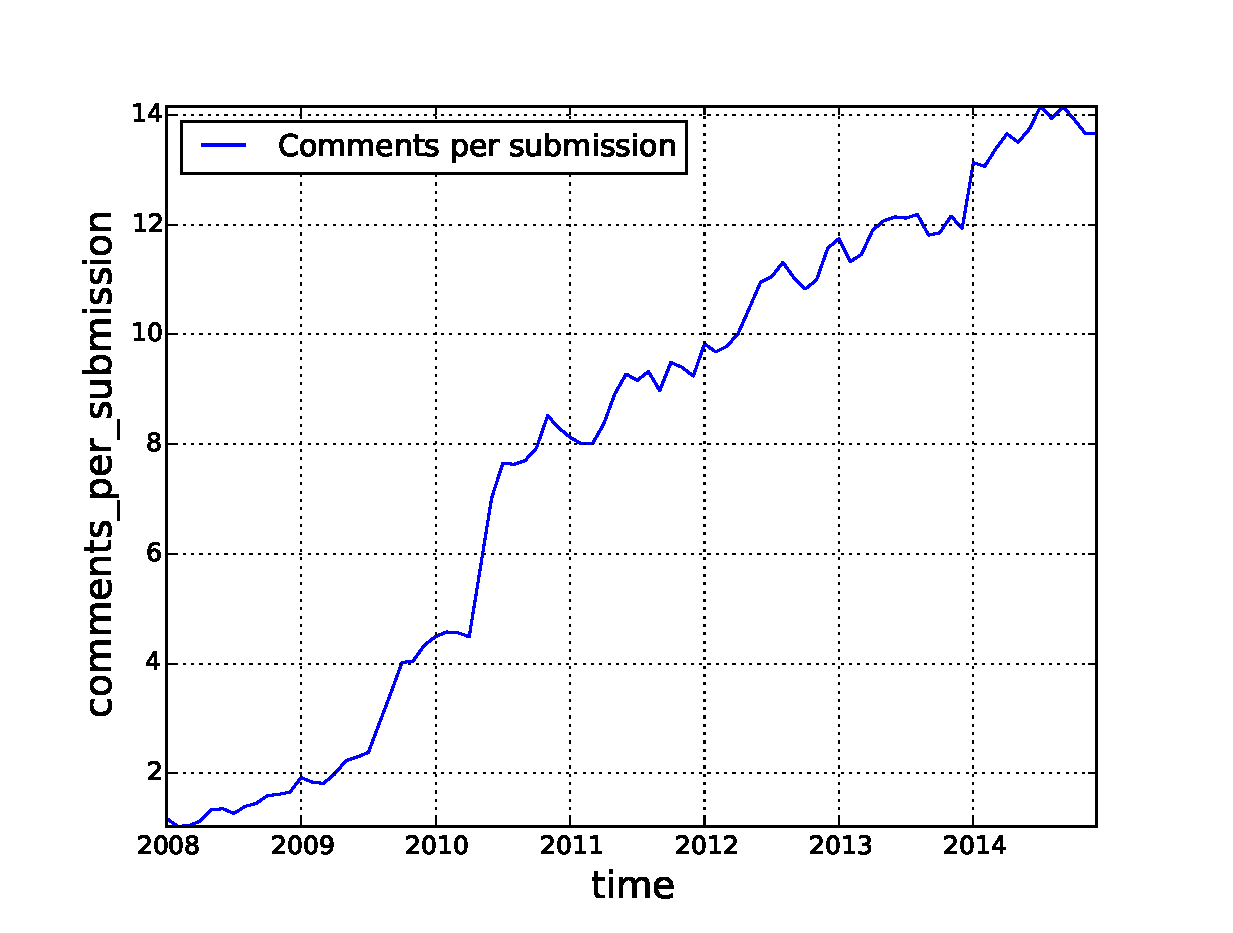
\includegraphics[scale=0.4]{./images/comments_per_submissions_over_time_total.eps}
%\caption{Comments per submission ratio for Reddit over time. We observe an overall increasing trend of comments for each submission. Notice that these should not be interpreted as how many comments each submission gets, but as how many comments users author for each submission --- submissions might get comments a long time after they are posted, by users from different years. This distinction becomes more important when we change the time referential and separate users by cohorts.}
%\label{fig:comments_per_submissions_over_time_total}
%\end{figure}

%% DC 12: Redundant if there's an overall line in the cohort graph.
%\begin{figure}[!tb]
%\centering
%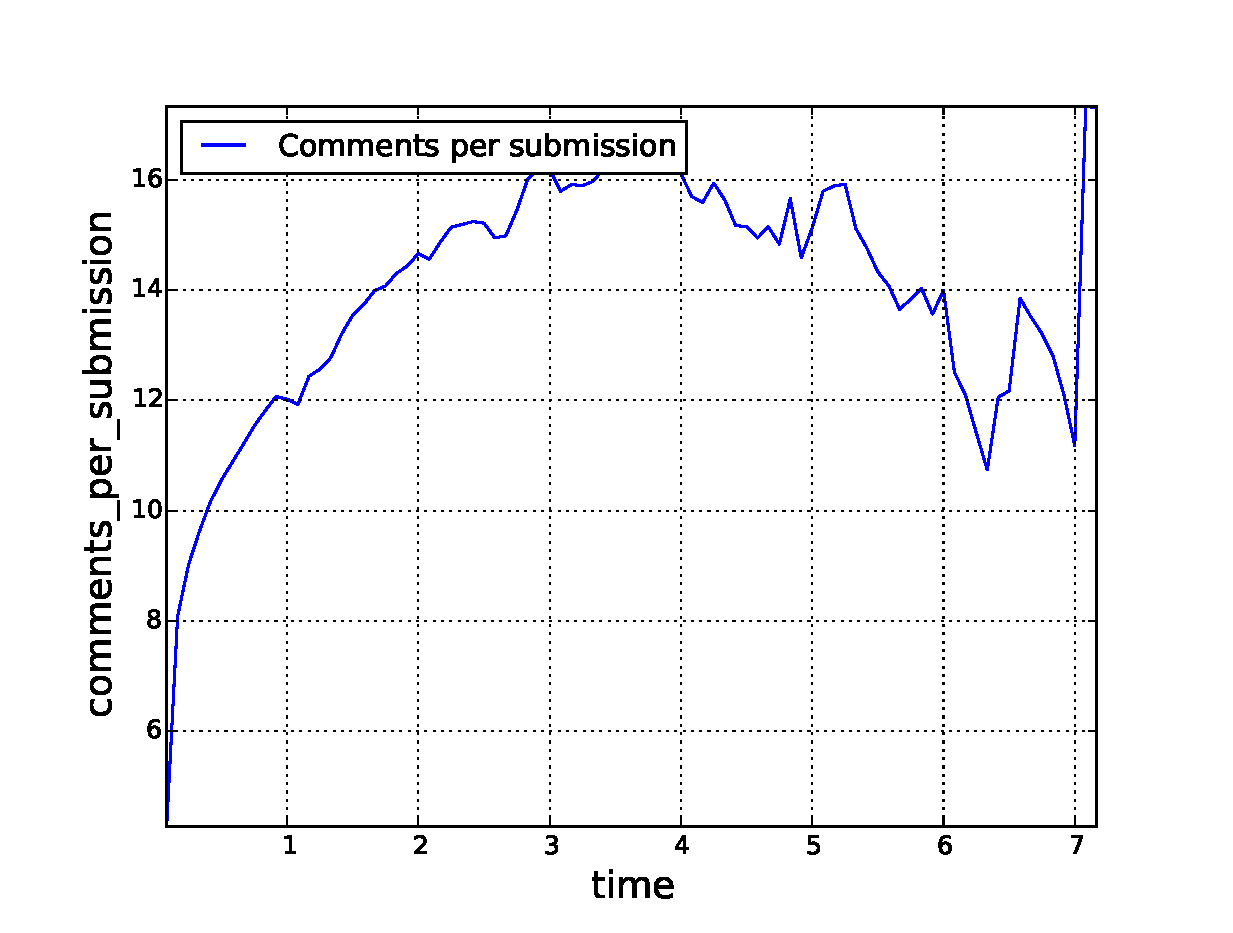
\includegraphics[scale=0.4]{./images/comments_per_submissions_user_ref_total.eps}
%\caption{Comments per submissions ratio from the user referential. This should be interpreted as how many comments a user makes for each submission in their x-th year of existence. We observe an interesting overall trend that peaks between 3 and 4 years of existence. This, however, does not mean that users will necessarily decrease their behavior as they live longer, but that given that a user has survived for x years, what is his/her comment per submission ratio likely to be.}
%\label{fig:comments_per_submissions_user_ref_total}
%\end{figure}

%We have found that segmenting users and subreddits by cohorts on the years that of the first comment highlights significant differences of behavior and help us to understand how Reddit changed over these years.


%Table 1: Number of distinct users that authored comments and submissions segmented by the year of the first post of the user. The Total numbers are based on posting data from 2007 until 2014, corresponding to our full dataset. The Oct 1st, 2014 onwards numbers are based on the last 3 months of data we have, and we consider this as the current, active Reddit.
%
%
%Table 2: Number of distinct subreddits segmented by the year of the first post of the user. The Total numbers are based on posting data from 2007 until 2014, corresponding to our full dataset. The Oct 1st, 2014 onwards numbers are based on the last 3 months of data we have, and we consider this as the current, active Reddit.

%Table indicates that Reddit grew significantly from 2007 until 2012, practically doubling the number of new users per year for each of these years, with similarly significant growth in subreddits. Although the most expansive growth happened in the first years, more than half of the registered users are from the last 2 years, and their behavior is significantly different than previous users, impacting in the overall behavior of the community. For instance, users from the 2014 cohort have a higher tendency to make submissions instead of comments, in contrast with all the previous cohorts.

%\begin{figure}[!tb]
%\centering
%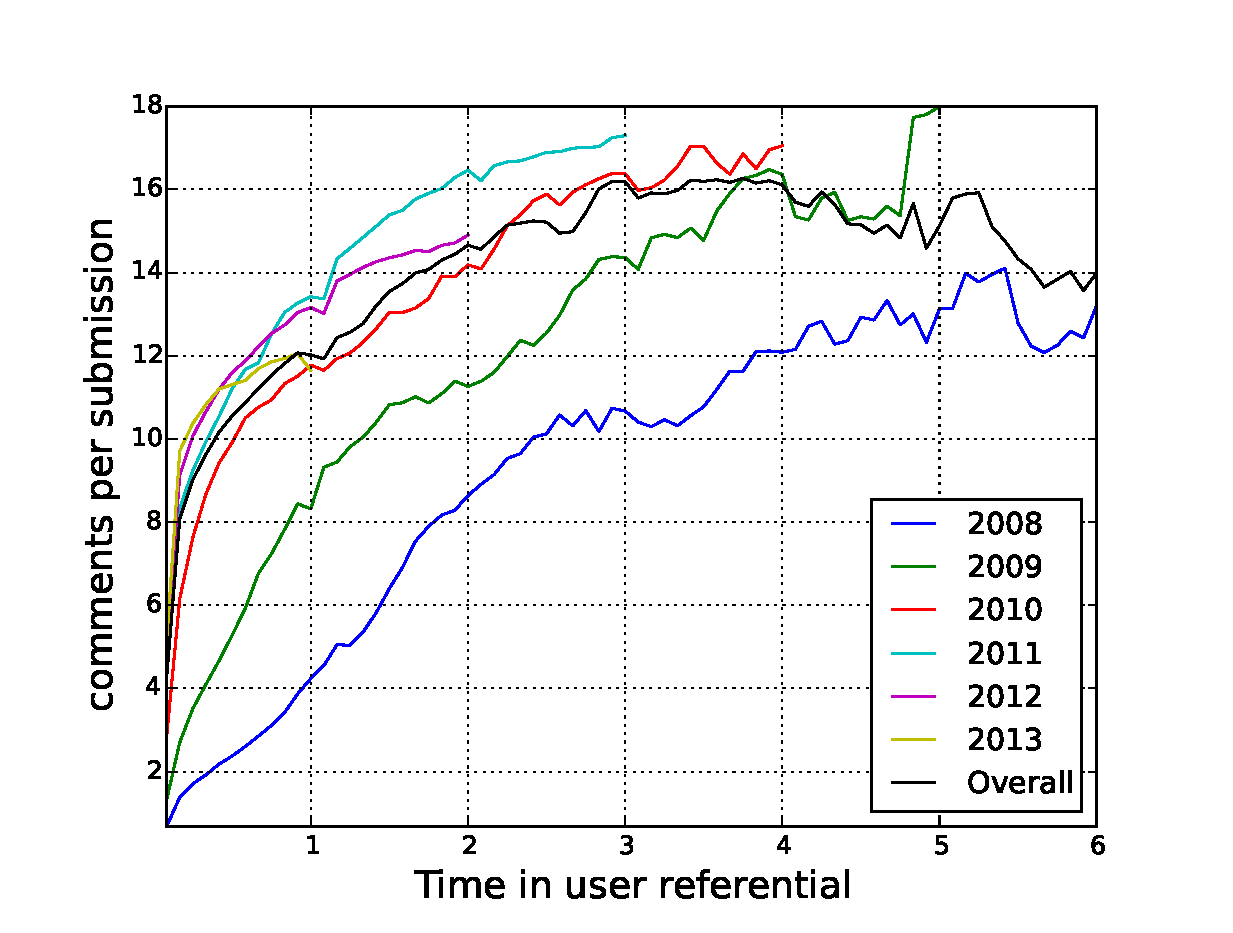
\includegraphics[scale=0.4]{./images/comments_per_submissions_cohorts.eps}
%\caption{Comments per submissions cohorted by user creation year. Here we observe that, unlike the total aggregated graphic, all users are are increasing the number of comments per submissions, but latter cohorts show a much higher level of comments per submissions than earlier cohorts. This brings the initial part of the aggregated user-referential curve up, while the end of the curve consists only of users from the latter cohorts that preset an lower ratio. It is also important to notice that, as these curves move to the right, less comments and submissions exist in the bins, for there are less users that survived for such long periods. This results in some spiky behavior in the rightmost end of some curves due to the reduced amount of data. Just as with the previous user-referential cohort curves, we can not distinguish solely based on this graphic if users are increasing their commenting behavior or if the users that do not comment die earlier. Figure \ref{fig:comments_per_submissions_for_surviving_year} help us to answer this question.}
%\label{fig:comments_per_submissions_cohorts}
%\end{figure}


% DC 12: I'd probably get rid of the survival part for space and coherence.  We're doing analysis that focuses on the surviving users and should just be clear on that and own it.  We can talk about the limitations of that, and questions around how to measure survival, in a discussion maybe.
%\subsection{Users' Survival}
%
%The simplest definition of an active user in Reddit is to set a threshold date and define that every user that posted after that date is an active user and users that do not show any kind of behavior are ``dead''. This, however, is a limited interpretation of how users decide to stay or leave the network, specially if we want to analyse how this behavior changed over time. Also, since our users might always come back to the network at a later time, they might be ``reborn'', that means we have right censored data.
%
%To account for these, we look at a one year window of time for each user. This way, we avoid the right censored data and the possibility that a user might have come back to the network at a later time. Given this, we segment users by their cohort and define that users active in the last 3 months of this one year window are active users. Based on this data manipulation, we present the Kaplan-Meier (cite) survival curve in Figure N.
%
%\begin{figure}[!tb]
%\centering
%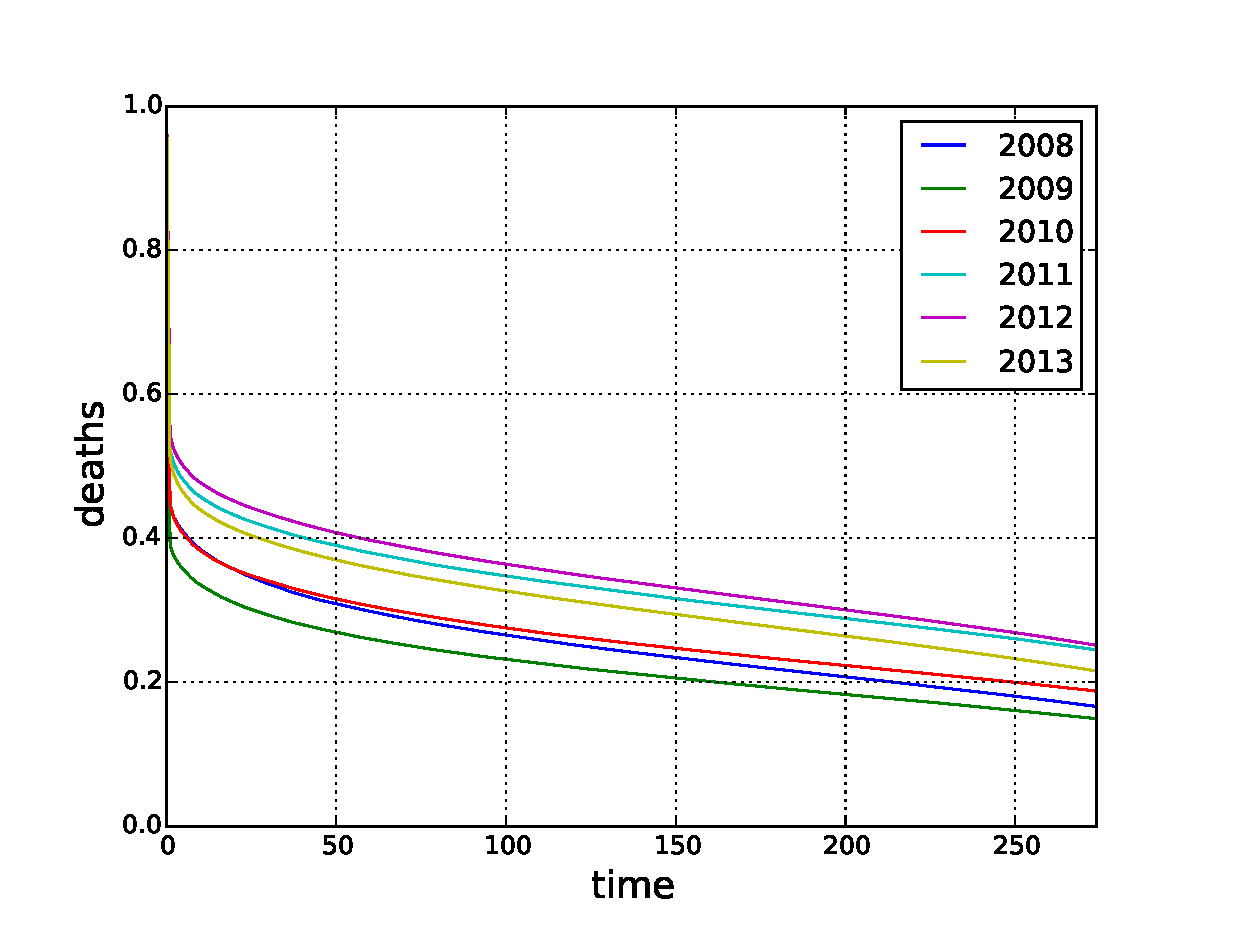
\includegraphics[scale=0.4]{./images/kaplan_meier_users.eps}
%\caption{Kaplan-Meier estimator for one year of posting behavior for each user. Users for which the last posting day was in the first nine months of the one year window are considered ``dead''. This graph shows the percentage of surviving users per number of days since it first posted segmented by the cohort year the user joined the network.}
%\label{fig:kaplan_meier_users}
%\end{figure}
%
%As previously mentioned, Reddit shows a significant number of ``single time users'' that only post once in their existence. This can be seen in the initial drop in the first day. An interesting thing to see is that, although different cohorts level in different survival values, the ``user decay'' is similar throughout all of them. Not only that, but there is a general trend for older cohorts to die faster than younger ones. One possible explanation for that is that early Reddit still lacked in content, with few subreddits to submit and few submissions to comment. This could lead to a higher number of users that did not stayed around after their initial impressions. 
%
% Sam 10: This Figure (c)an go if we don't want/can't give a better explanation regarding survival. It is quite common for survival works to have the hazard plot, although I don't fully understand the values myself.
%\begin{figure}[!tb]
%\centering
%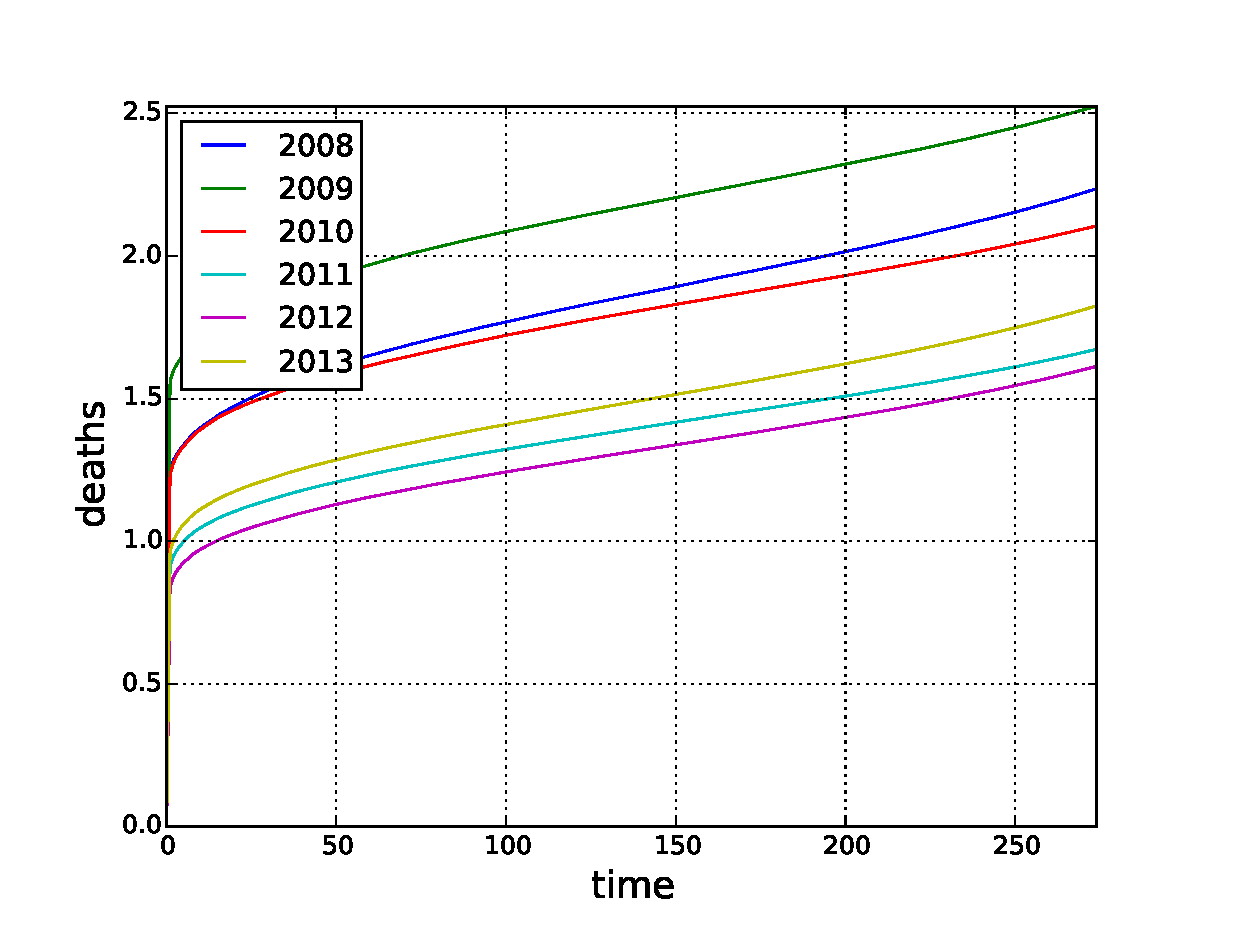
\includegraphics[scale=0.4]{./images/nelson_aalen_users.eps}
%\caption{Nelson-Aalen empirical hazard estimation for the users survival. This curves show the pointwise probability of a user to die in time.}
%\label{fig:nelson_aalen_users}
%\end{figure}
%
% DC 12: Have to stop here.


%%%%%%%%%%%%%%%%%%%%%%%%%%%%%
%%% DC 15: Moving some commented out stuff from above to here for readability in the main line of tex.

%\begin{figure}[!tb]
%\centering
%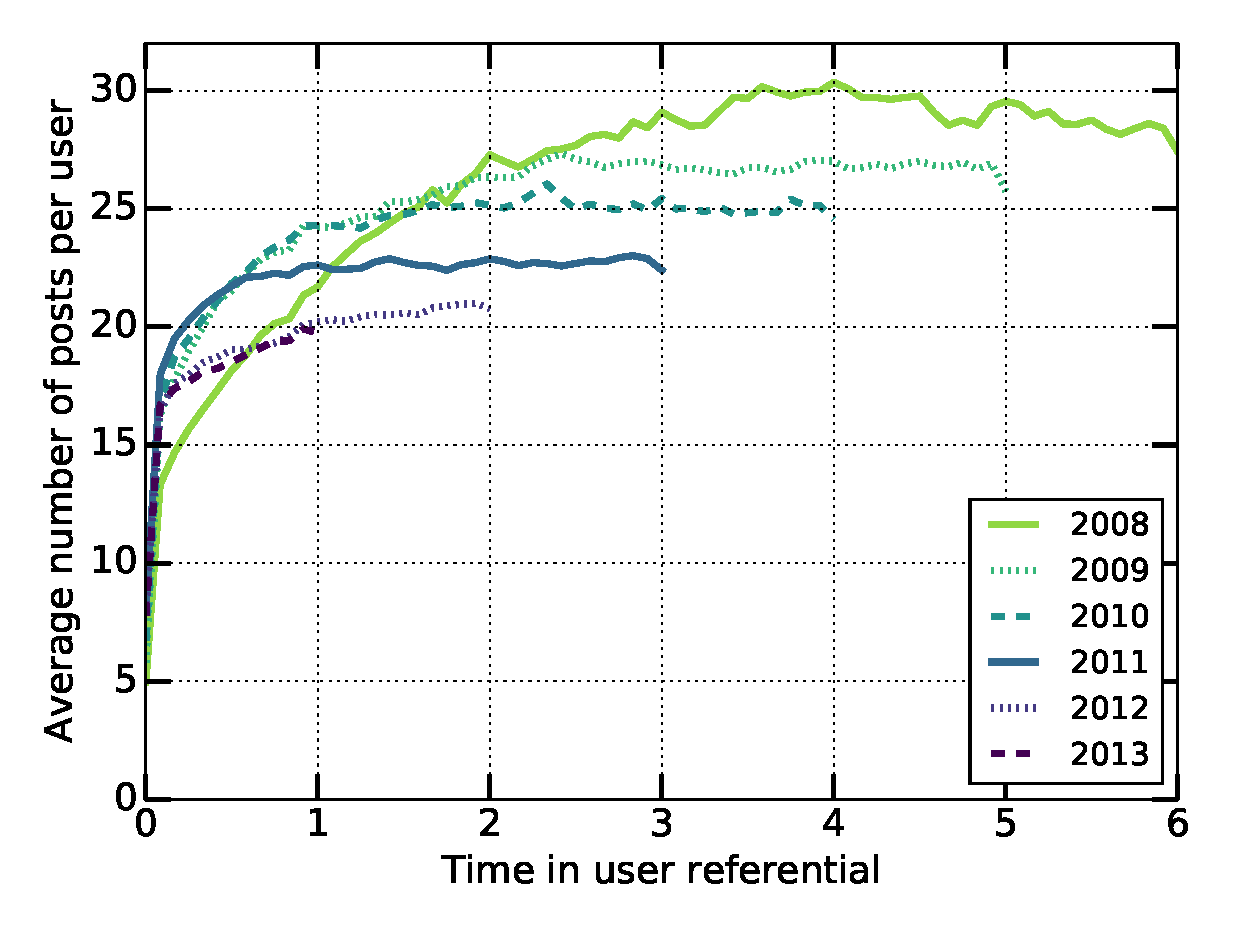
\includegraphics[scale=0.4]{./images/avr_posts_per_user_cohorts.eps}
%\caption{Number of posts per active user for  the overall set of users and cohorts on the user creation date. The x-axis is the time from the user creation referential, i.e., each message creation time is measured in terms of when the user was created. Each tick is one year and we discretized time by month --- the n-th bin holds messages the user wrote in the n-th month. Since we are looking at the user time referential, you can understand this as the surviving users after x time. An interpretation of this says ``users that survived x time are posting on average y messages''. Here we see that, although the 2008 cohort level at a higher value, the evolution of the number of posts took a longer time to increase. The other cohorts seem to follow a more regular pattern after the first year: older users that survived the first year post more on average than younger users that survived the first year. Since we are talking about surviving users, it is not clear from this figure whether these curves increase because the ``low posting users'' are dying earlier or because the users are actually increasing their activity as they live on. To differentiate these cases, Figure \ref{fig:avr_posts_per_user_for_surviving_year} shows, for each cohort, the average posting for users grouped by the number of years they survived in the cohort.}
%\label{fig:avr_posts_per_user_cohorts_relative}
%\end{figure}
%% DC 12: The captions need to be longer than one line, but on average shorter than this.  The first set of figures probably wants longer-than-usual captions to explain what's going on (and you do good to not re-explain things later), but the analysis probably has to go to the body text. 
%\begin{figure}[!tb]
%\centering
%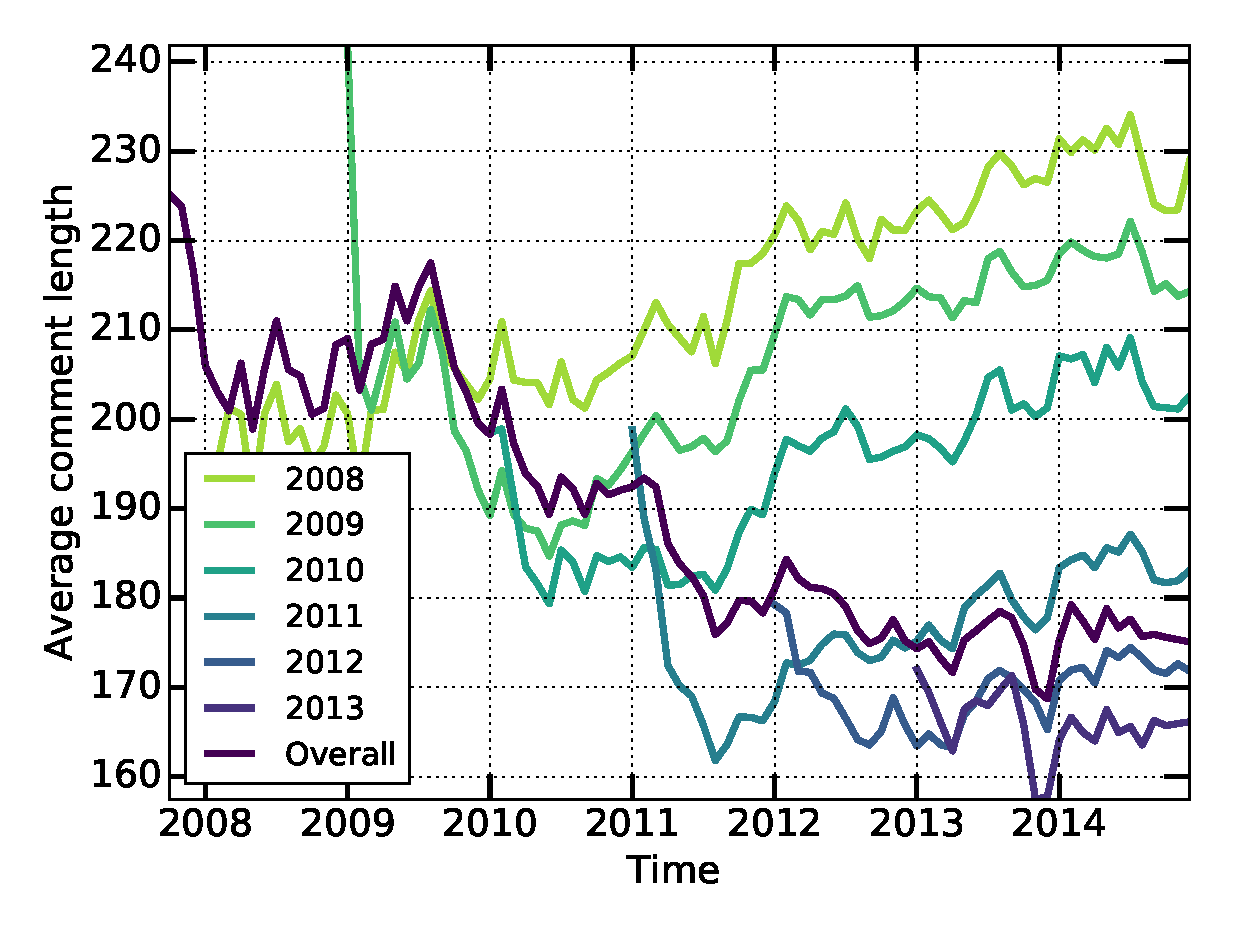
\includegraphics[scale=0.4]{./images/avr_comment_size_over_time_cohorts.eps}
%\caption{Average comment length over time for cohorts on user creation time superimposed over the trend for the total of users. Here we observe how the early existence for each cohort has a reasonable agreement with the overall trend. This might indicate how the new users might be just adopting the community norms regarding comment length.}
%\label{fig:fig_label}
%\end{figure}

%% DC 12: If we're going to focus our attention on the median, then we should re-shoot the graphs to also look at the median.
%% Sam 12: Re-doing everything based on median right now is not really feasible right now. I can redo the table, that is easy.
%\begin{figure}[!tb]
%\centering
%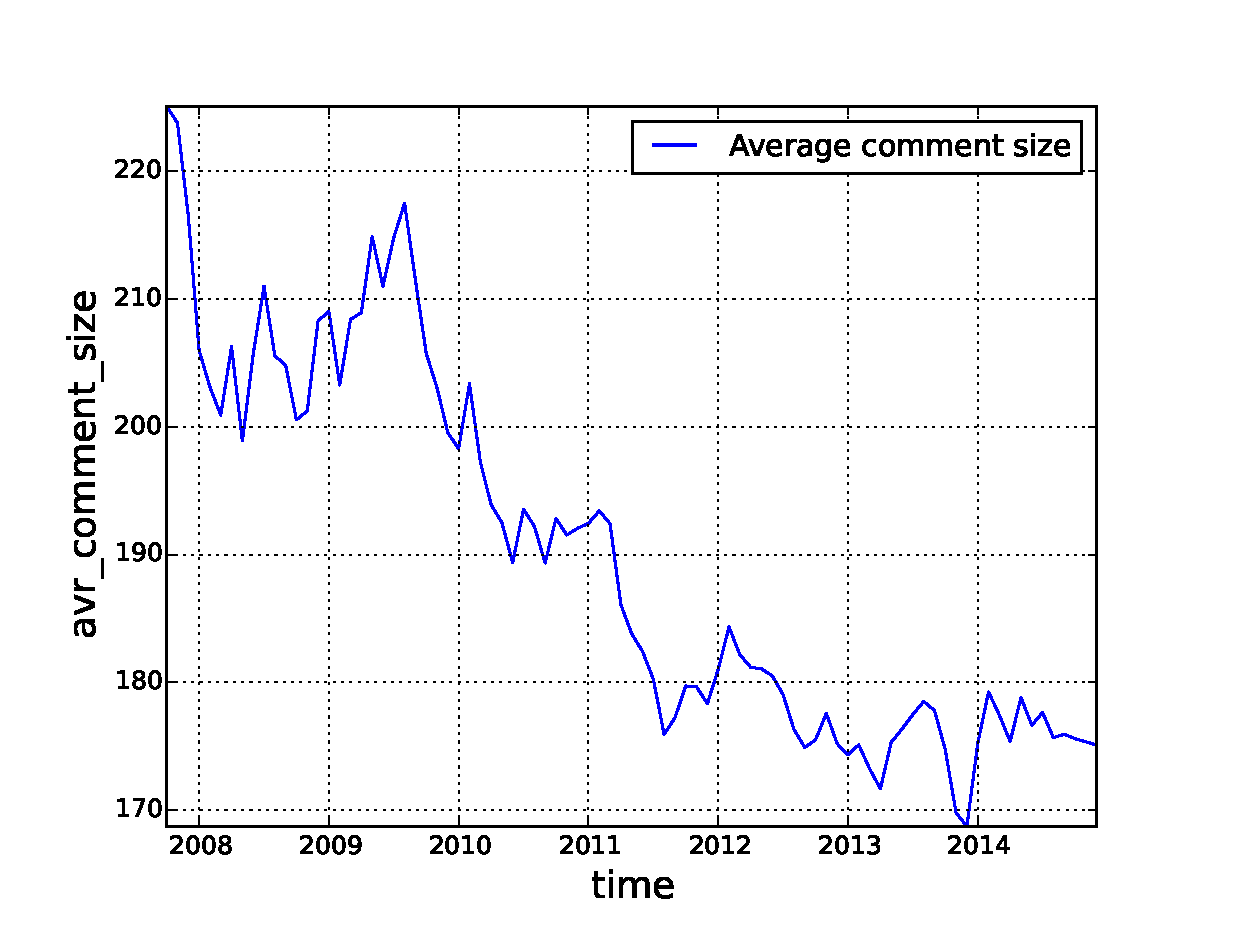
\includegraphics[scale=0.4]{./images/avr_comment_size_over_time_total.eps}
%\caption{Average comment size (number of characters) over time for the Reddit network. We observe that there is a decreasing trend for the average comment size. This means that users, on average, are making smaller comments in Reddit as time passes. This, however, hides important aspects of user behavior over time and does not mean that users, as they survive in the network, write smaller comments.}
%\label{fig:avr_comment_size_over_time_total}
%\end{figure}

%% DC 12: Assuming that we start doing the combined cohort and overall graphs, this figure is no longer needed.
%\begin{figure}[!tb]
%\centering
%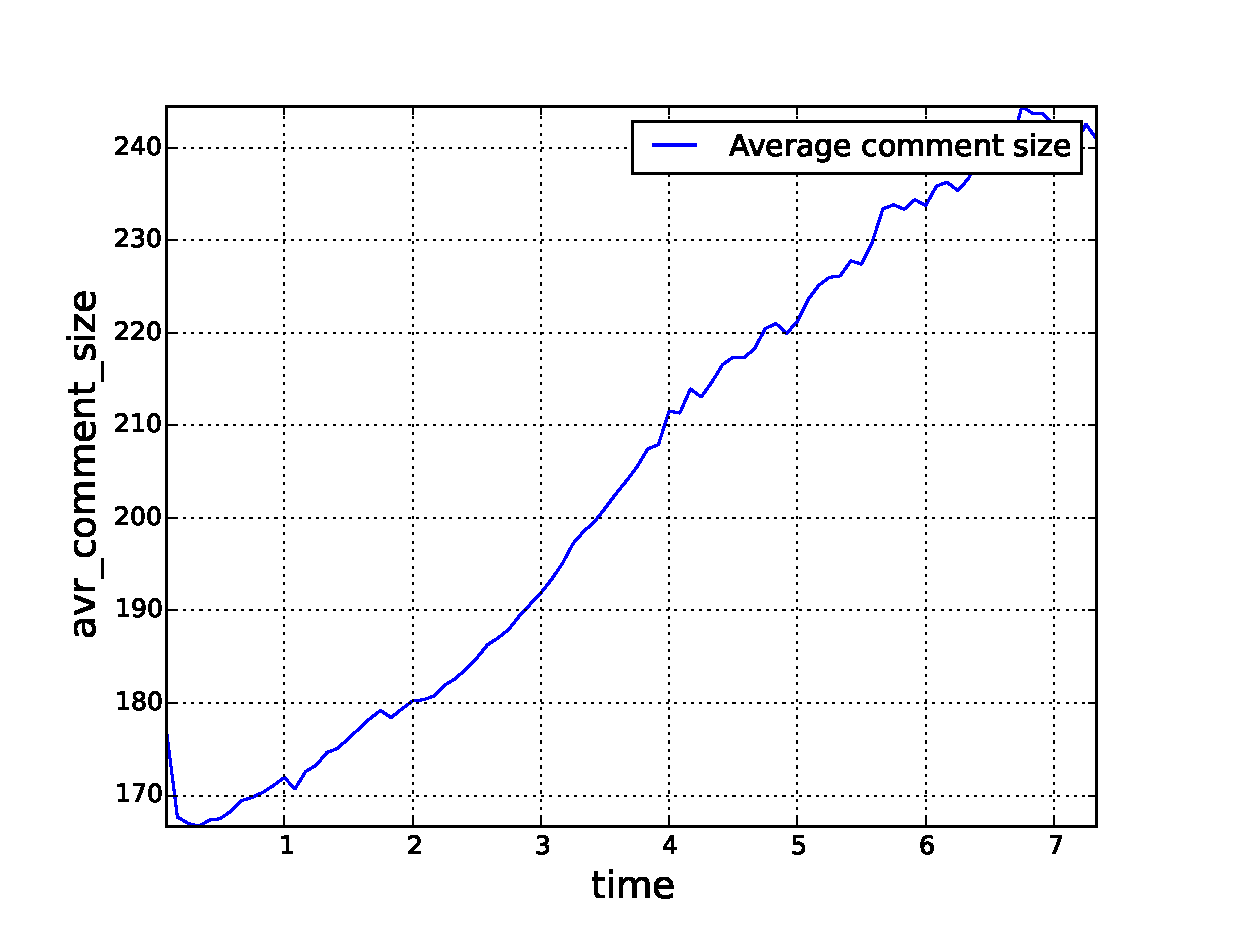
\includegraphics[scale=0.4]{./images/avr_comment_size_user_ref_total.eps}
%\caption{Average comment size from the users time referential. This shows that comment length made by users increase for users that lived longer in the network, save for a small decrease in the initial time. This, however, is also not enough to say that we should expect the average size of the comments in the network to increase since the users that survive write longer comments.}
%\label{fig:avr_comment_size_user_ref_total}
%\end{figure}

%% DC 12: This first one still has no real justification: where is the theory or empirical evidence that demographics is what's going to drive this?
%Some possible explanations for this difference in the starting points could be that older users are, again, sampled from a different demographics that is more committed and willing to spend more effort into developing their virtual identity. 
%% DC 12: Again, this is an interesting speculation, but one that's not at all connected to these data.  When papers try to make these kinds of process speculations that aren't supported by either theory or evidence, they usually are not believable.  In some worlds this one could come in a discussion maybe.
%Also, it could be that it is a natural evolution of the community, as older users have taken most of the main space of interests when it comes to creating new subreddits and starting these communities, new users have it all already made and sometimes might feel intimidated or not motivated to create new topics or communities that already exist or that are less likely to compete with the existing ones. In a way, these new users could behave more as lurkers, while the older users are the ones that laid the foundation of Reddit.

% DC 12: If we're going to focus our attention on the median, then we should re-shoot the graphs to also look at the median.
%\begin{figure}[!tb]
%\centering
%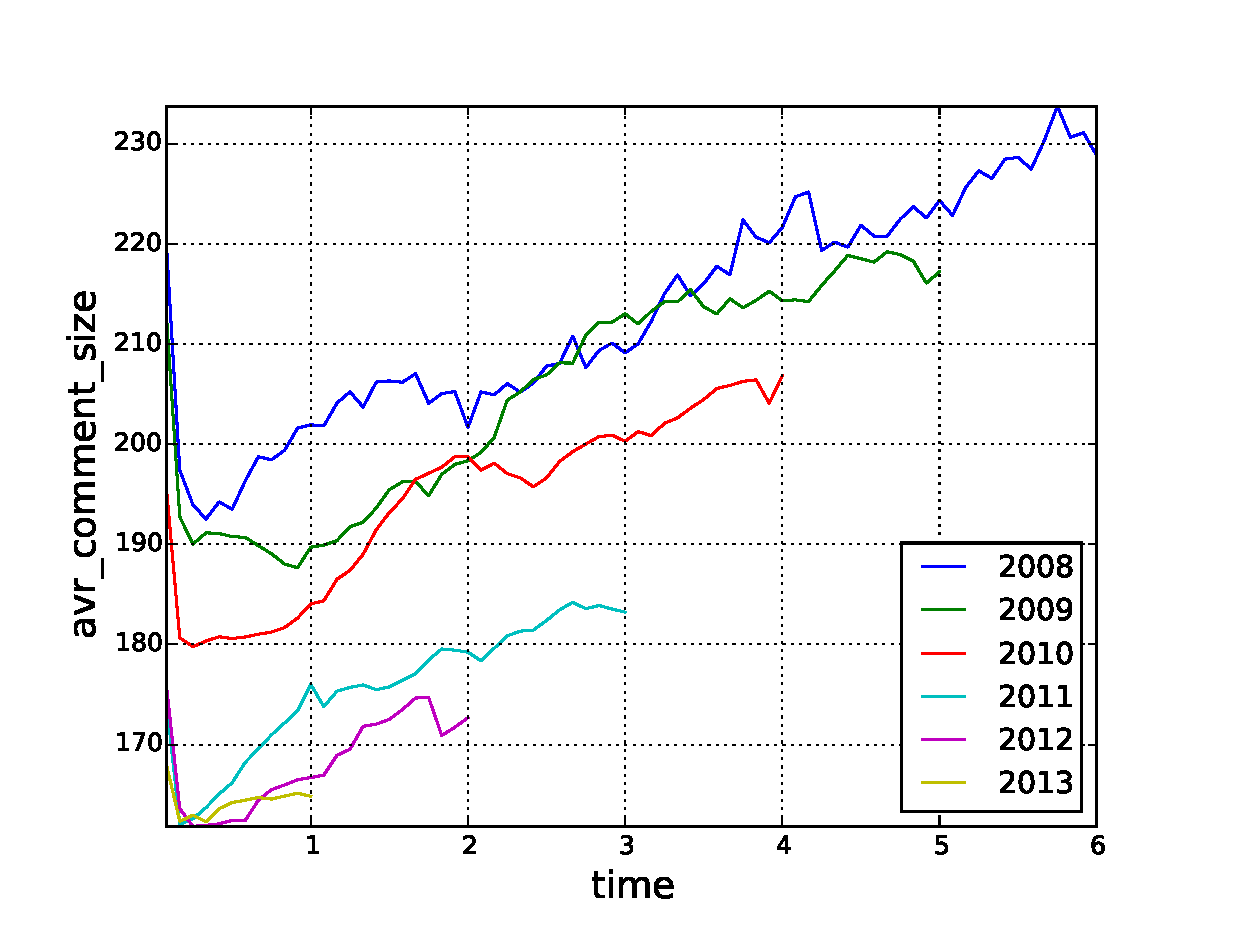
\includegraphics[scale=0.4]{./images/avr_comment_size_cohorts.eps}
%\caption{Average length of comments from the user time referential segmented by user creation cohorts. This figure start to explain why we see different trends in the overall network comment length and user referential overall comment length. It shows that, as users come from latter cohorts, they start from a lower commenting length average compared the the earlier cohorts. This, together with the fact that Reddit is growing exponentially in terms of users means that \textit{we have an influx of users that make smaller comments than the previous generations}, although even for them, as they survive, they make longer comments. Just as for the users' posting average, we can not distinguish based on this graphic alone whether users that make smaller comments leave the network earlier or they indeed write longer comments as they survive. Figure \ref{fig:avr_comment_length_for_surviving_year} sheds some light on this question.}
%\label{fig:fig_label}
%\end{figure}

%% DC 12: 2008 and 2009 awfully noisy here, possibly worth deleting on this one; the 2010-2013 are the money shots here for me.  The first point has already been made by the overall, but the second point is a really interesting observation.
%% The y-axes _have_ to be on the same scale for all of the subfigures, though; this "repeated multiples" style demands that because people are going to expect to be able to visually compare them.
%% They should also be shot at medians if you like median better.

%% DC 12: I am confused by the comment, because I don't know either the percentage like or the wikipedia example parts.
%Sam 9: Still unclear if we should calculate the proportion above and bellow the median of the previous year to have a ``percentage like'' number just as in the wikipedia example. I would like to have this set up as similar as possible as the easiest reference people can find about the subject. A little bit going up by the end, although for some analysis including 2014 and 2007 is a problem, I don't necessarily think it gets in the way here, should we get rid of them?
%\begin{table}[htbp]
%\centering
%\tabcolsep=0.11cm
%\singlespacing
%\fontsize{7pt}{8pt}\selectfont
%\begin{tabular}{|>{\raggedright\centering\arraybackslash}m{1.5cm}|c|}
%\hline
%Year & Median \\ \hline
%2007 & 114 \\ \hline
%2008 & 103 \\ \hline
%2009 & 103 \\ \hline
%2010 & 96 \\ \hline
%2011 & 91 \\ \hline
%2012 & 89 \\ \hline
%2013 & 87 \\ \hline
%2014 & 88 \\ \hline
%\end{tabular}
%\caption{Evolution of the median throughout the years for the whole Reddit dataset.}
%\label{tab:simpson1}
%\end{table}


%% DC 12: I think subreddits and joint_cohorts probably get merged since they're largely explained by the same phenomenon of default subreddits for new users.
%\section{Subreddits}

\subsection{Subreddits Activity}

One way to look at reddit is as a multi-community social network. Each subreddit can be considered as a semi-independent community, and as such, we can study the evolution of these communities based on time, cohorts and survivability.  A number of other online communities have similar properties, with tighter (Wikiprojects, enterprise social network discussion groups) or looser (Wikia, StackOverflow) interdependence between the individual sub-communities.

One of the initial question we can ask is how is the number of posts in these surviving communities evolving? One thing to be aware here though is that this variable is likely to be sensitive to the ration of active users per active subreddits. If we imagine that users don't change their posting patterns rapidly, and increased number of users per subreddits implies in an increased number of posts per subreddit. The overall number of users per subreddits, however, seems fairly stable throughout the years.

Figure N shows the evolution of number of posts per active subreddits in time for subreddits created between 2008 and 2013. We can observe that the average number of posts per subreddit increases over time. Since the ratio of active users per subreddit remains relatively stable, one could imagine that subreddits are receiving more posts throughout the time.

\begin{figure}[!tb]
\centering
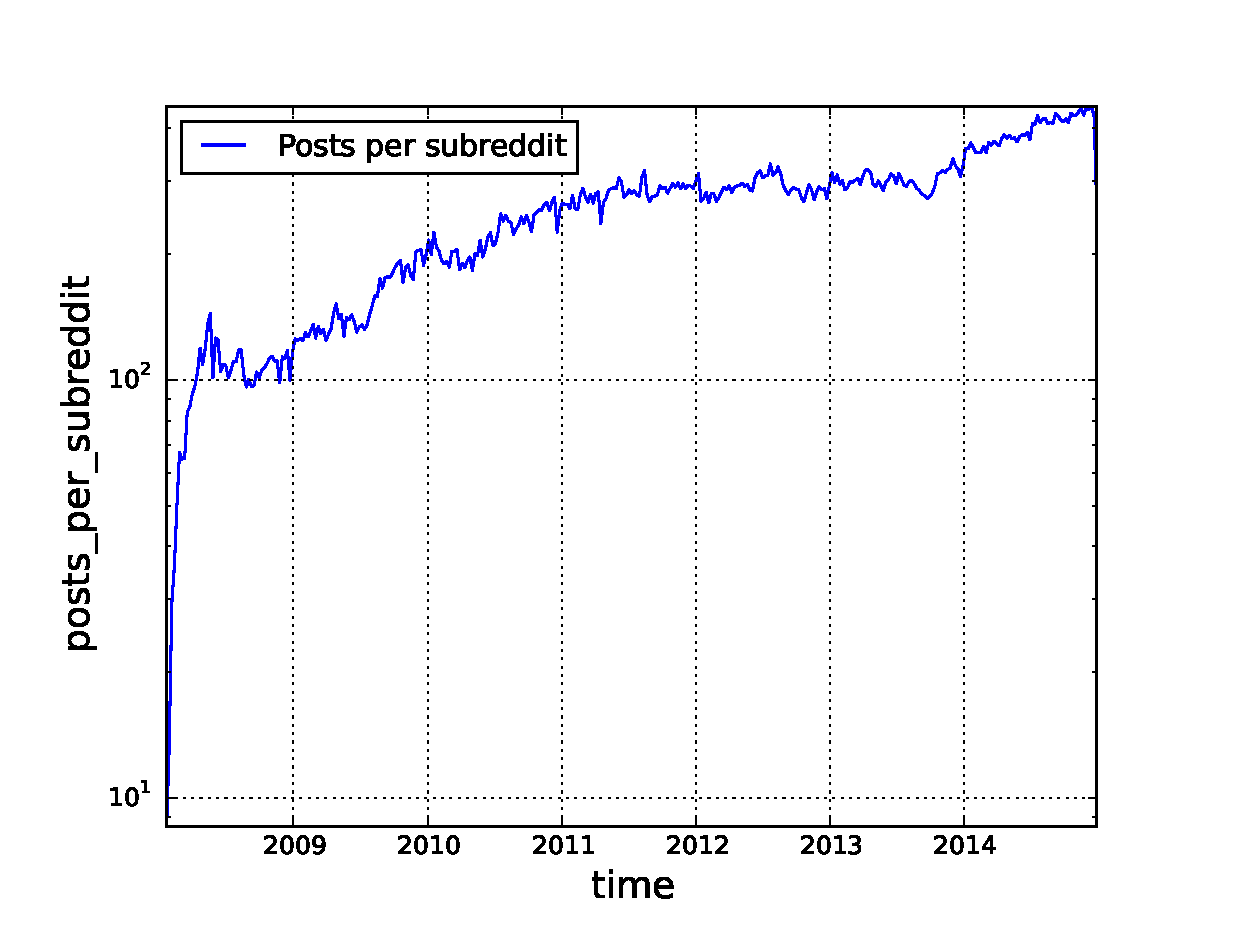
\includegraphics[scale=0.4]{./images/posts_per_subreddit_over_time_total.eps}
\caption{Caption}
\label{fig:posts_per_subreddit_over_time_total}
\end{figure}

To better understand how correct is this conclusion, we cohort the subreddits in time. We can observe that the majority of posts in reddit are made in 2008 subreddits, and the posting averages for this cohort dominates the total posting average for the whole social network. Also, we notice that for most points in time, the number of posts per subreddits increases as we move to older cohorts. This, however, is not sufficient for us to conclude that these communities are evolving in different ways, since subreddits from older cohorts had more time to consolidate their reach and popularity and most of the ``likely to die'' subreddits that bring the average number of posts down in newer cohorts are still alive.

\begin{figure}[!tb]
\centering
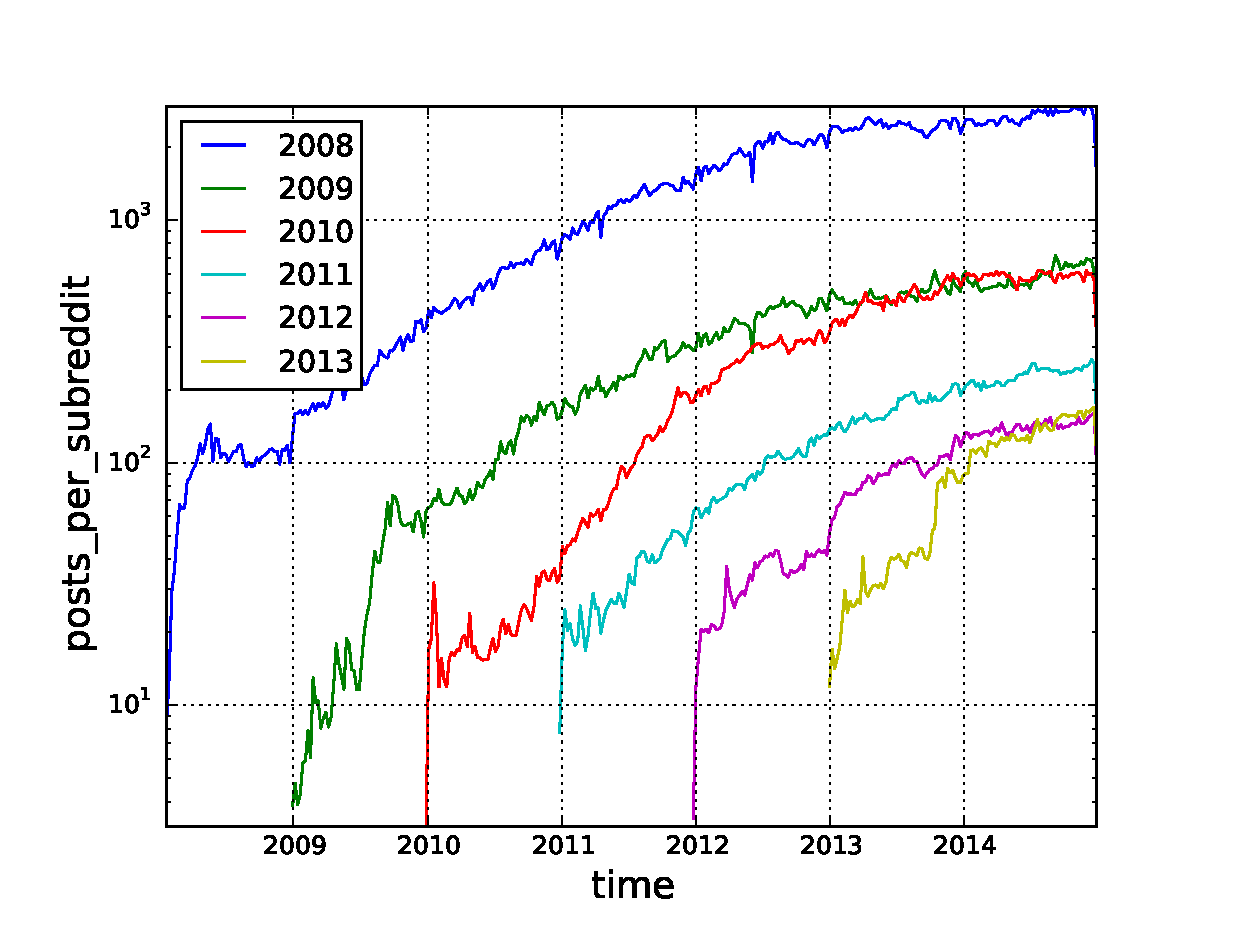
\includegraphics[scale=0.4]{./images/posts_per_subreddit_over_time_cohorts.eps}
\caption{Caption}
\label{fig:posts_per_subreddit_over_time_cohorts}
\end{figure}

To properly compare these communities starting from the same baseline, we evaluate every posting time according to the subreddit creation time (fists post ever made in the subreddit). The x-axis then becomes the time the subreddit has lived, grouped by cohort. This approach reveals a general trend of subreddits from newer cohorts stabilizing in a lower posting average than older cohorts. This, however, does not hold true for the 2009 and 2010 cohorts, although they stabilize in very similar levels, and for the 2013 cohort, for which we have only one year of data in the overlap for all subreddits.

\begin{figure}[!tb]
\centering
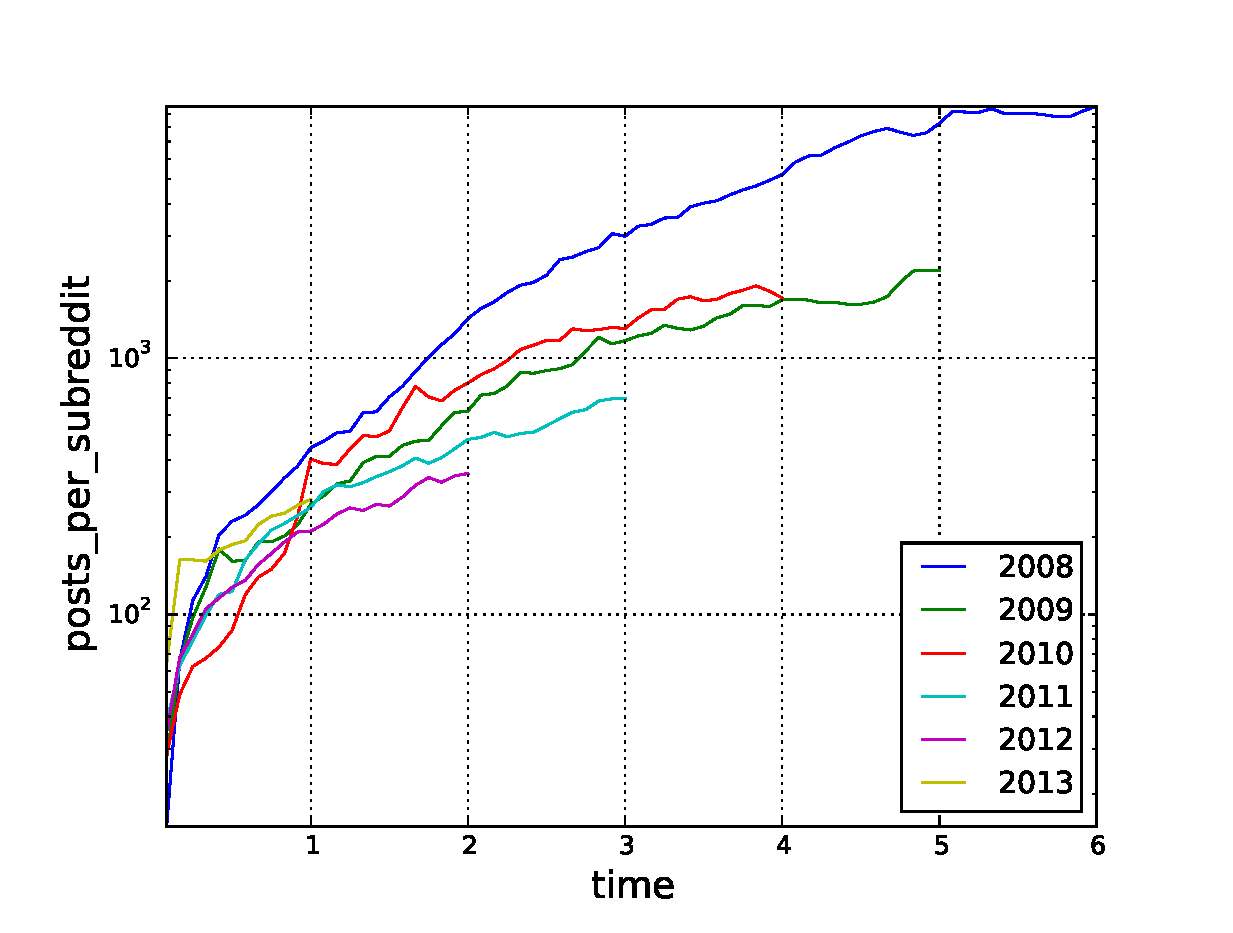
\includegraphics[scale=0.4]{./images/posts_per_subreddit_cohorts.eps}
\caption{Caption}
\label{fig:posts_per_subreddit_cohorts}
\end{figure}

Assuming that subreddits that survive have, on average, a higher number of posts than the ones that do not survive, part of the higher levels of posting for the older cohorts could also be explained by a faster ``death rate'' of the low posting subreddits. Therefore, the faster the number of posts per subreddit grows, the faster the non-fit subreddits are being eliminated.

\subsection{Subreddits' Survival}

Similarly to what we did for users, we look in a one year time window for the last post that was created for each subreddit and define as subreddits that died as the ones that the last post happened in the first nine months of the one year window. The Kaplan-Meier curve is shown in Figure N.

\begin{figure}[!tb]
\centering
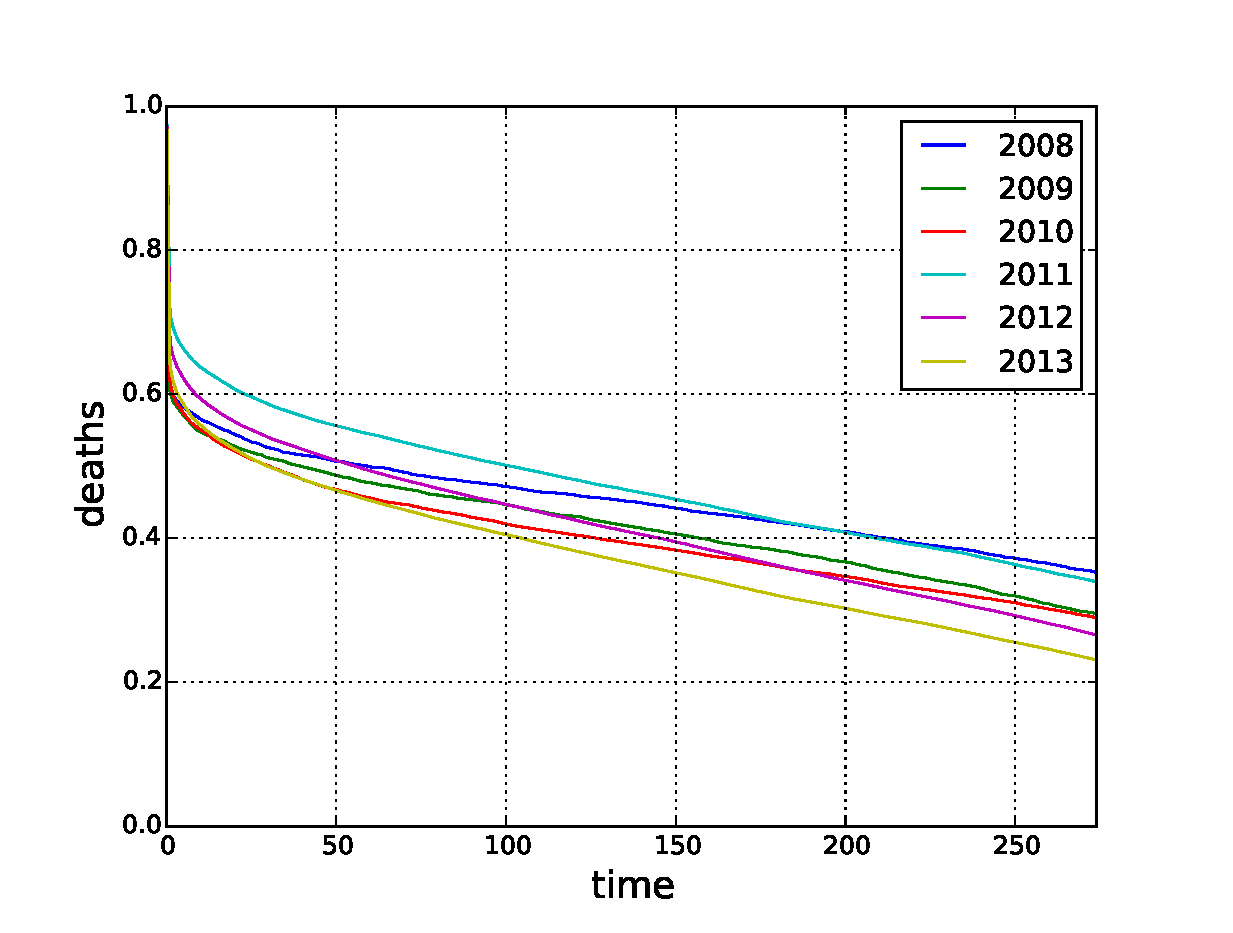
\includegraphics[scale=0.4]{./images/kaplan_meier_subreddits.eps}
\caption{Caption}
\label{fig:kaplan_meier_subreddits}
\end{figure}

In this survival curve, we also observe that there is a significant number of subreddits that survive only through the first day, just as seen with the users, although the proportion in this case is not as high as the users . Also, unlike the users, there are significantly differences in the ``decay of subreddits''.

\begin{figure}[!tb]
\centering
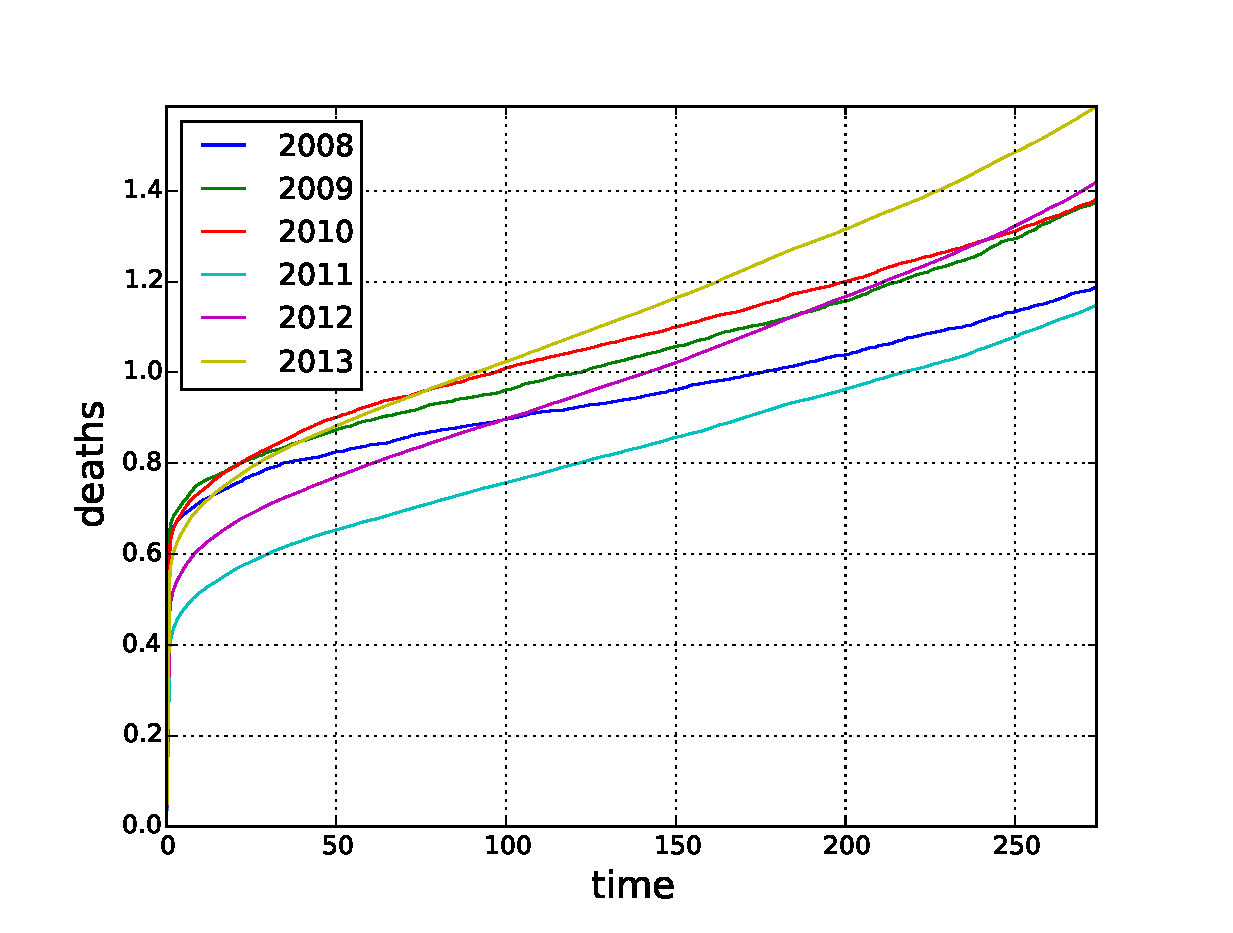
\includegraphics[scale=0.4]{./images/nelson_aalen_subreddits.eps}
\caption{Caption}
\label{fig:nelson_aalen_subreddits}
\end{figure}
\section{User Bias for Early Content}

\begin{figure*}[!tb]
\centering
\begin{subfigure}{.3\textwidth}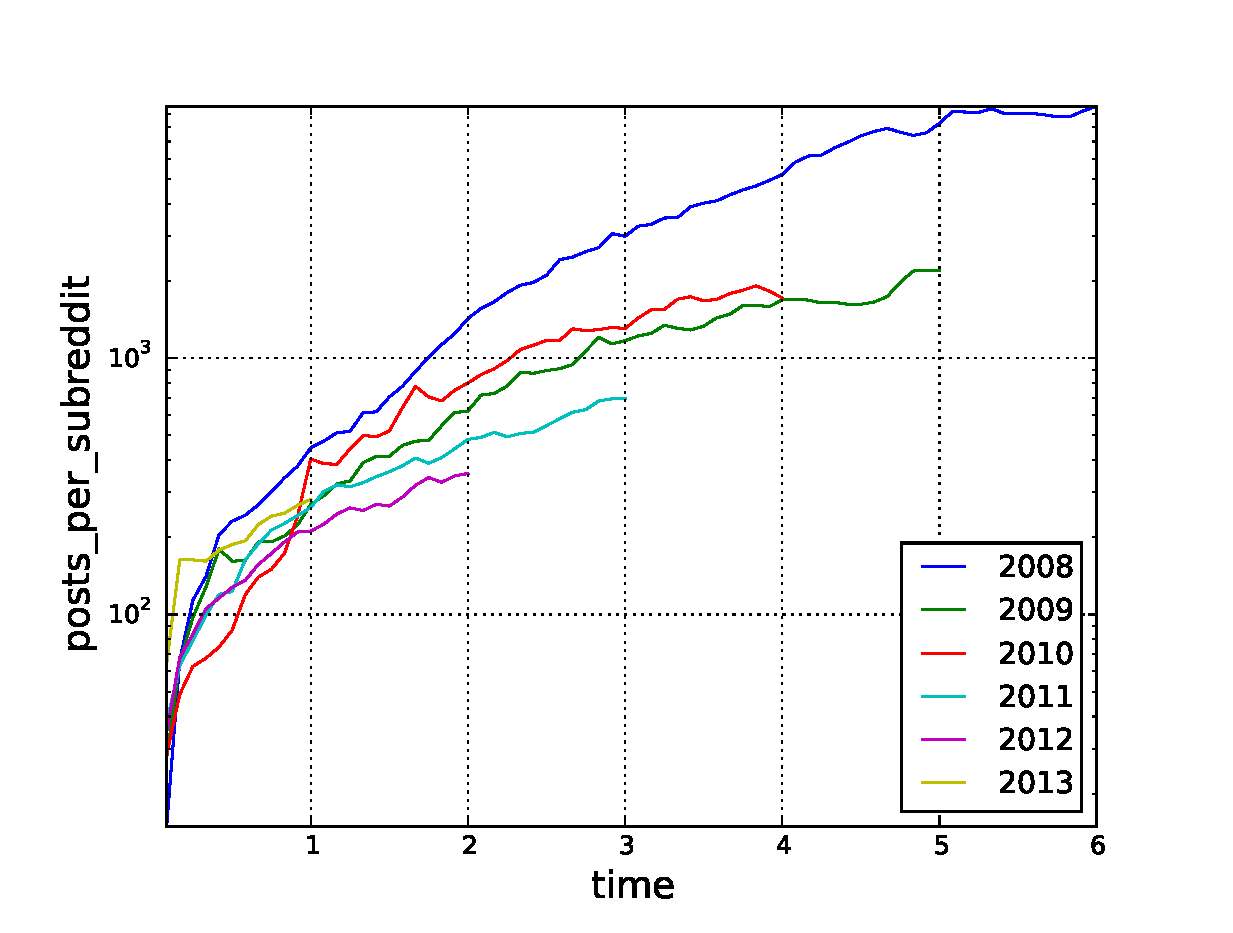
\includegraphics[scale=0.285]{./images/posts_per_subreddit_cohorts.eps}\caption{}\end{subfigure}
\begin{subfigure}{.3\textwidth}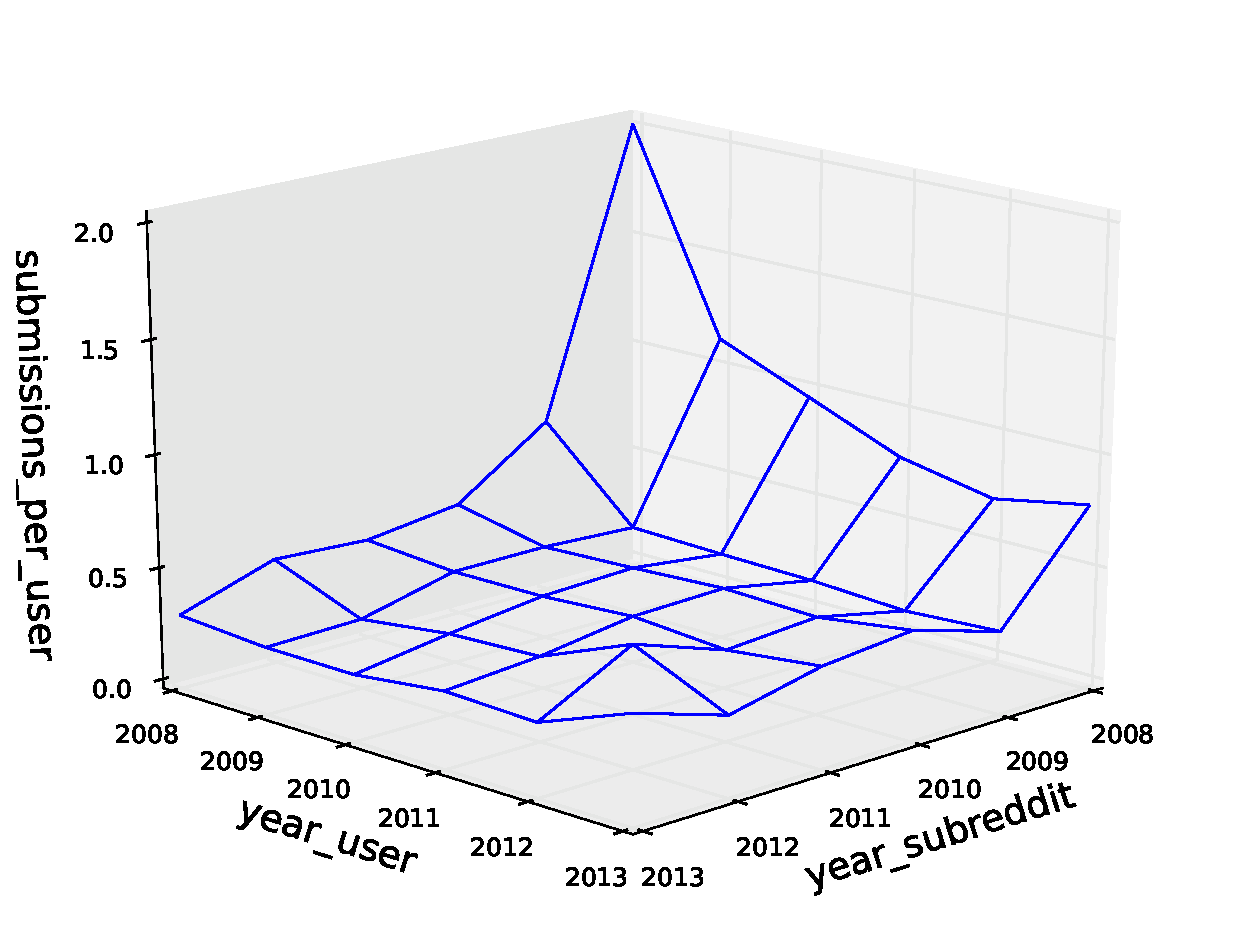
\includegraphics[scale=0.285]{./images/user_subreddit_submissions_cohorts.eps}\caption{}\end{subfigure}
\begin{subfigure}{.3\textwidth}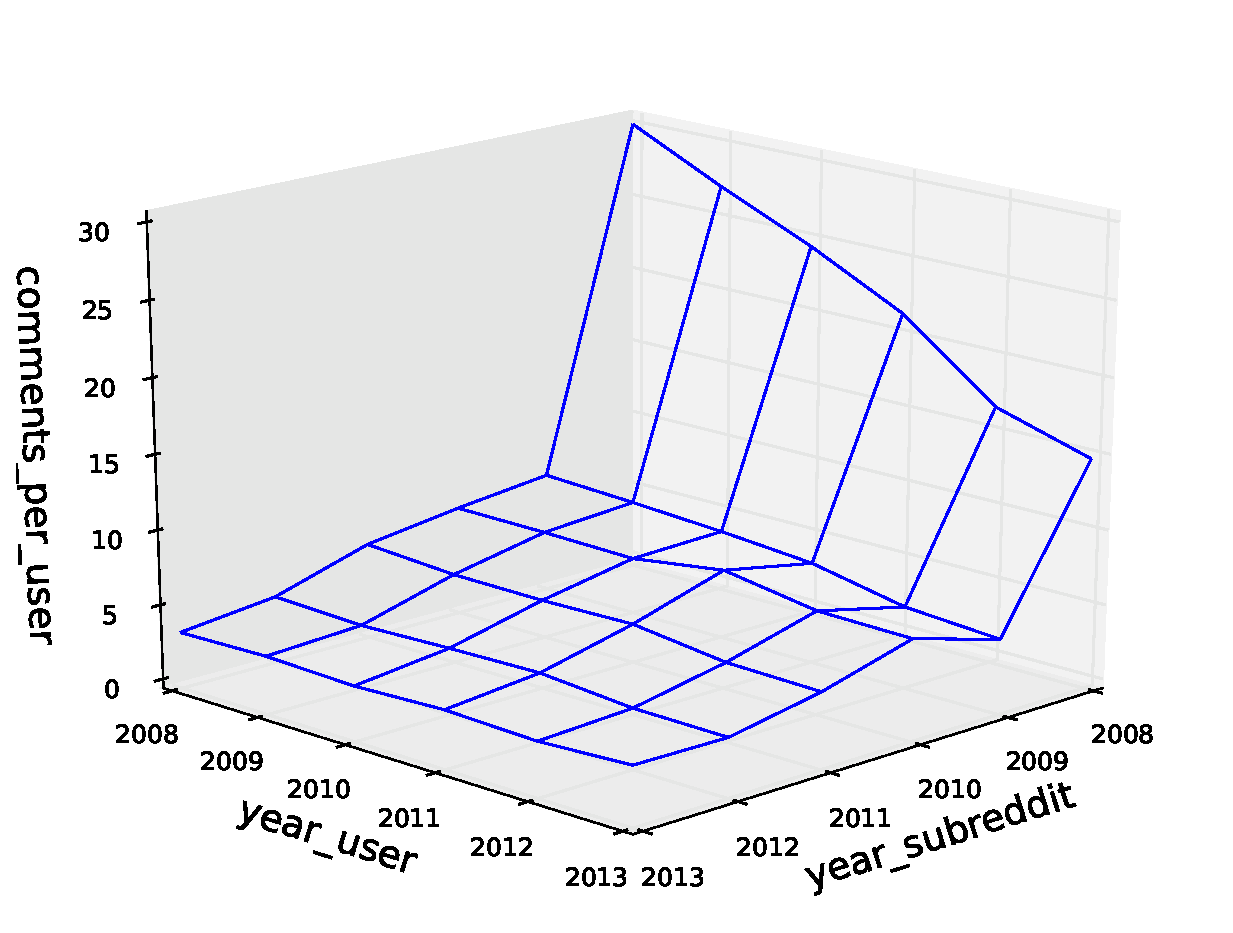
\includegraphics[scale=0.285]{./images/user_subreddit_comments_cohorts.eps}\caption{}\end{subfigure}
\caption{Figure a shows the monthly posts per surviving subreddit cohorted by the subreddit creation date (first post to the subreddit). Figure b and c shows, respectively, the number of submissions and comments per user in reddit for the last three months of 2014, segmented by user creation year and subreddit creation year. Each bin counts the number of comments or submissions based on the user and subreddit creation year and divide by the total number of active users created in that year.}
\label{fig:joint}
\end{figure*}

The cohort a user belongs to has a significant impact to the user posting behavior, but that does not give us a picture of how these users coexist in the current community or the communities evolution on time. An interesting hypothesis that we could imagine is that users from a particular cohort are more interest in the communities from a particular cohort. We now look at the interplay between user and subreddit cohorts. 

Figure \ref{fig:joint}a shows the number of posts in the subreddit-time referential for cohorts on the subreddit creation year. The most striking observation here is how 2008 subreddits are significantly more active than other subreddits for the same survived time. This led us to question what could be the process for this bias. One piece of evidence that we found that can significantly bias the user posting choices are the default subreddits a user is automatically subscribed upon creation \footnote{\url{https://www.reddit.com/r/defaults}}. These subreddits change over time and are said to be ``a set of highly popular communities that the administrators of this site feel would give the average person an interesting first experience'' \footnote{\url{https://www.reddit.com/wiki/reddit_101}}. Even if this set is defined only after the subreddits get popular, there might be a positive feedback that maintains the ``core subreddits'' as the most popular ones. We observe the bias for 2008 when we count each of the default subreddits set over time according to their creation year, seen in Table \ref{tab:defaults}.

\begin{table}[!tb]
\centering
\tabcolsep=0.11cm
\singlespacing
\fontsize{7pt}{8pt}\selectfont
\begin{tabular}{|>{\raggedright\centering\arraybackslash}m{1.5cm}|c|c|c|c|c|c|c|c|}
\hline
 & 2007 & 2008 & 2009 & 2010 & 2011 & 2012 & 2013 & 2014 \\ \hline
December 31, 2009 & 5 & 6 & 1 & - & - & - & - & - \\ \hline
October 18, 2011 & 3 & 14 & 2 & 2 & - & - & - & - \\ \hline
October 19, 2012 & 2 & 16 & 3 & 2 & 2 & - & - & - \\ \hline
July 17, 2013 & 2 & 15 & 2 & 1 & 2 & - & - & - \\ \hline
January 1, 2014 & 3 & 14 & 2 & 2 & 3 & - & - & - \\ \hline
April 19, 2014 & 3 & 13 & 2 & 2 & 2 & - & - & - \\ \hline
May 7, 2014 & 4 & 23 & 6 & 5 & 4 & 7 & 1 & - \\ \hline
\end{tabular}
\caption{Count of subreddits per creation year for each default set of.}
\label{tab:defaults}
\end{table}

Figures \ref{fig:joint}b and \ref{fig:joint}c show a more current picture of reddit. While submissions in Figures \ref{fig:joint}b are in general more skewed towards 2008, it is even more striking that users from 2008 submit even more. This might be due to the fact that these surviving users play a much more central role in these communities (moderators or key contributors) since they are more likely to be there from the start (relative to the total number of users from the cohort that are still active), as we see evidence in Table \ref{tab:mods}. Figures \ref{fig:joint}c show that comments are even more skewed than submissions towards 2008 subreddits. The tendency, however, is of decreasing commenting behavior for the earlier user cohorts (we have seen that users from earlier cohorts are posting less, which justifies this decrease).

\begin{table}[!tb]
\centering
\tabcolsep=0.11cm
\singlespacing
\fontsize{7pt}{8pt}\selectfont
\begin{tabular}{|l|c|c|c|c|c|c|c|c|}
\hline
 & 2007 & 2008 & 2009 & 2010 & 2011 & 2012 & 2013 & 2014 \\ \hline
Moderators & 757 & 1182 & 2108 & 4085 & 8059 & 9340 & 6868 & 4262 \\ \hline
Percentage & 8.52 & 6.02 & 5.2 & 3.91 & 2.54 & 1.5 & 0.82 & 0.18 \\ \hline
\end{tabular}
\caption{The first lines show the absolute number surviving users that posted as moderators in each cohort. The second line shows the relative percentage to the surviving users for the same cohorts. Were considered active the users in the last three months of 2014.}
\label{tab:mods}
\end{table}

%% DC 15: Worked to beef this up and try to integrate stuff in the "future work" section. 

\section{Discussion}

In this section we discuss some of the processes that might explain our observations, and how they connect to other literature.  We're not arguing here that we know the answers; instead, we see these as interesting avenues for future work.  

\subsection{Why are newer ``active'' users less so?}

We have seen that users from later cohorts have a lower posting average than in earlier cohorts. 
One plausible explanation is that users self-select: users that find Reddit early in its life are also more likely than average to be those who will be attracted to it. Previous work has shown that online book reviews have a self-selection bias, where people who are more likely to like (or promote) the book review it earlier, leading to a positive early bias in an item's life \cite{Li2008}.  In Reddit's case, this would mean that the mixture of users joining in the early stage of the community would be disproportionately likely to be the most active ones and the latter ones are more likely to be less active. 

Another plausible hypothesis for later cohorts having a higher number of less active users could be that, over time, Reddit has accumulated an increasing number of valuable-but-small/niche communities.  The increased diversity might support a wider set of users in getting value, explaining the increased survival percentage.  The niche/smaller nature of newer communities might provide fewer opportunities to both submit and comment, explaining the lower average activity for surviving users. 

A third hypothesis is that Reddit overall is becoming more about consumption and voting on content rather than producing it.  Older users with contribution norms continue to contribute; newer users tend to provide audiences and feedback.  High-resolution voting data could be a real boon in understanding if this is true.

\subsection{Why are comments getting shorter?}

We also observed that overall, comment lengths are getting shorter over time.  

One hypothesis is that users are being shaped by an ``initial value problem''. We can imagine that users as they join the network, tend to produce content according to the norms of what they see \cite{Kooti2010, Danescu-niculescu-mizil2013}.  The observed behavior of the comments length for the users in Reddit is a initial drop, followed by steady increase as the user survives. If the starting point for the initial drops are taken as the average of the network, that is what is observed by the user in the network, the initial drop would place each cohort starting at lower levels than the previous one.  Figure~\ref{fig:comment_length}a presents some support this hypothesis: the initial month of each cohort year, which consists of data only from users who joined in that month, is quite close to the overall line from the prior month.  

Another hypothesis advanced by community members \footnote{See \url{https://www.reddit.com/r/TheoryOfReddit/comments/1a7aoj/retracing_the_evolution_of_reddit_through_post/  }.} is that reddit's karma system favors shorter comments.  That is, people can get more upvotes for a given amount of effort by writing more, shorter comments.  This could be directly measured even with the available data, and might be the start of a very interesting line of future work that tries to model strategic posting and attention distribution behavior in Reddit. 

\subsection{Why do comments per submission increase?}

We also saw that comments per submission increase over time for surviving users, and that this is most dramatic for users who join earlier.

One process hypothesis is that this is because early in Reddit's life, there simply weren't as many submissions to comment on, meaning that people who wanted to be active contributors more or less had to submit in order to do so. 
As the community grew, more content became available, making information seeking more valuable---and perhaps increasing the value and ease of commenting. 

This question of ease and value might be more general, and tie to our earlier observations about self-selection and karma accumulation.  Most users in social networks are known to be lurkers: users that only seek information and passively observe, not engaging and contributing to the network \cite{Rafaeli2004, Nonnecke2000}.  Consumption is valuable and easy, and in reddit, some contributions are easier than others: reading is easier than voting; voting is easier than commenting; commenting is easier than submitting.  Only users for whom finding and submitting comment is relatively easy or relatively valuable are likely to be frequent submitters or ``power users'' \cite{Panciera2009, Kittur2007}---and we suspect such users are more likely to be ones who found Reddit earlier on and stuck with it when it was relatively small.

\subsection{Limitations and Future Work}

In this paper we focused our attention on behavior attributable to specific users, which in this dataset meant submissions and comments.  As with many analysis that focus on visible behavior, this means we miss important phenomena.  In particular, we discount lurkers despite their known importance as audience members \cite{Nonnecke2003} and potential future contributors \cite{Ridings2006}.  Many lurkers likely vote, and thus lurking may be even more important in a context like Reddit where votes affect content visibility and provide explicit markers of attention and reputation.  

However, the dataset does not have information on individual voters or timestamps, just the aggregate number of votes a post had received at the time of the crawl, making it impossible to effectively treat them as activity measures and ways to understand the behavior of those who voted.  The existing voting data might be much more useful, however, in addressing questions that involve predicting a given user's future behavior based on whether and how other users respond to a user's early contributions \cite{Joyce2006,Sarkar2012}

Another blind spot that focusing on visible behavior can induce is our emphasis on active users.  This is a reasonable view of the community that focuses on what is happening, but our results should all be interpreted in the context of ``given the set of active users at any given time''.  Applying these results to questions that require considering all users would be a mistake.  

We did, implicitly, consider survival in the analyses that broke cohort down by survival time; we see careful thinking about what it means to ``survive'' in a community as an interesting problem in its own right.  Potentially, users' ``breaks'' from the network can influence both our results and other analyses that assume users depart on their last visible day of activity. 
Focusing on activity also fails to account for actual deletion in many contexts.  In Reddit, activity from users is marked with a username of ``[deleted]'' (which we were able to ignore after realizing that one author had millions of comments!), but in some contexts, such as Wikipedia articles that are deleted, edit behavior on those articles do not show up in many data dumps.

These questions of how to define active users and dead users and distinguishing patterns of behavior seems an interesting venue to pursue. Better definitions of ``active'' and ``dead'' users might allow us to characterize the burstiness of their behavior.  Some users might only interact with the network in some specific occasions while some users might have a much more uniform pattern; in Wikipedia, the practice of leaving temporarily is so common it is called a ``wikibreak''. Understanding how your network fares in terms of user burstiness is essential to understand how the users use the network and to shape the user experience.  A better definition of ``death'' would allow us to investigate the ``rebirth'' of users, that is, users that come back to the community.  Rather than an annoying right censorship statistical problem, it might pose a much more central issue, as a community's survival might not depend only in its ability to attract and retain users, but also in the ability to ``resurrect'' old users.

\section{Conclusions}

This work highlights the importance of taking time into consideration when analyzing users' evolution in social networks. We do so by cohorting the users based on their creation year. Although simple, this approach provides evidence of significant differences between methods that account for time with methods that do simple overall analyses.  We also analyze the evolution of users and communities from a shifted time referential: considering the time of an action in relation to the user creation date. This also reveals unexpected phenomena that we would otherwise not notice.

From the user perspective, we found that user posting activity for surviving Reddit users is actually significantly higher than a naive average would suggest, that older users who survive are considerably more active than younger survivors, and that these newer users are unlikely to catch up.   Controlling for survival, we also found that users have a stable level of posting activity over time (with slightly decreasing patterns) and the percentage of surviving but low-activity users is increasing in the younger cohorts.  

Similarly, we analyzed user effort based on average comment length. We found that, while the overall average in Reddit seems to decrease, users actually write longer comments as they survive, no matter when they joined.  Still, later cohorts of users that joined the network are writing smaller comments; their greater number leads to this version of Simpson's paradox, where where the overall average decreases while the series for each individual cohort increases. 

%% DC 15: Restate this in slightly more general terms if you can.
Finally, we analyze the type of activities users engage, differentiating comments and submissions. 
We found that users with a higher comments per submission ratio are more likely to survive longer in the network. More than that, this behavior changes as the users survive---particularly for the early cohorts. Users change their comments per submissions patterns, and their main mechanism to do so seems to be replacing their submitting by commenting behavior, since their posting activity remains stable.
%We observe that users from 2009, 10 and 11 are the main commenters in Reddit and that cohorts from 2010 onwards have a very similar evolution. 2008 and 09 cohorts, however, changed significantly their behavior as the network evolved.  
We also discussed a possible explanation for this observation based on commenting being partially an information seeking task with an associated effort between lurking and submitting. This made it less likely in early Reddit, in which content was not as available as in later years.

Both our and work and its limitations suggest fruitful directions for better understanding of users' evolution in both Reddit and online communities in general, directions we hope inspire other work in this area.  



%% Sam 15: Section gone
%\subsection{Why the bias to 2008?}
%
% Sam 14: Still have to work on this one.
%Were we expecting different results? Defaults? Core consolidation?
%These observations allow us to conclude that, in the case of Reddit, there are key subreddits that were created in 2008 that are the main focus of attention of all the users, although this is decreasing as new users join the network. Our hypothesis would not hold true in this case. This, however, might not hold true for other social networks, in which the communities or the content at the time at which users join the network might be their main focus of attention, highlighting again the importance of performing a cohort based analysis.


%% DC 15: I now actually don't believe this hypothesis, given that more new users stick around.  It _might_ be made part of a 3B hypothesis related to the one above, but I think we have enough that we can leave this off. 
% A fourth argument is based on cumulative advantage, status, and attention-seeking: surviving users from earlier cohorts might be more capable of producing content that gets attention from other users.  This would lead to them getting more comments and votes for their content, and people who get positive attention are more likely to return and contribute \cite{Halfaker2009, Choi2010, Sarkar2012}.  

%% DC 15: I wouldn't mind if you resurrect this section, but I feel like we've got plenty here now. 
%Although many observations were made regarding Reddit, the main goal of this paper is not to study Reddit in depth. Therefore, many observations still remain without an explanation. Being aware that latter cohort users decrease the size of their comments and tend post less allow us to question the nature and motivation of these users.  Are users commenting less because newer users they are less interested into engaging with other user or are they simply ``lazier'' and writing is becoming less attractive for the newer generations? If it is a matter of writing being a less preferred method of communication, could Reddit improve its users' interactions providing alternative ways to post media, such as pictures, audio and video? These are some questions that we can ask and needs further investigation of the data, and might evolve into new models of how user attention, effort and interaction in social networks are shifting through time.


%When we consider the evolution of the number of comments per submission, we observe that surviving users in earlier cohorts have lower ratios than later ones. Just as lurkers are the majority in the community and are attracted to it in search of information, we can imagine a set of users that are in the community in search of content and are willing to engage in commenting, but don't have the drive of a ``power contributor'' that make submissions and brings new content into the network. 


% This could be in part driven by attempts to nurture new subreddits.  Reddit also added a feature in 2008 that allowed people to create their own subreddits; after creating a subreddit, a natural goal is to make it appear active through frequent submissions, and until it reaches a critical mass of submissions, there is little to comment on.  (This second hypothesis assumes that subreddit creation is less frequent or less successful over time; this would be an interesting question to explore.)
 

	\section{Future Work}

Although many observations were made regarding Reddit, the main goal of this paper is not to study Reddit in depth. Therefore, many observations still remain without an explanation. Being aware that latter cohort users decrease the size of their comments and tend post less allow us to question ourselves about the nature and motivation of these users. Are users commenting less because newer users they are less interested into engaging with other user or are they simply ``lazier'' and writing is becoming less attractive for the newer generations? If it is a matter of writing being a less preferred method of communication, could Reddit improve its users' interactions providing alternative ways to post media, such as pictures, audio and video? These are some questions that we can ask and needs further investigation of the data, and might evolve into new models of how user attention, effort and interaction in social networks are shifting through time.

One interesting question that recurrently arises when we were performing survival analysis was regarding the users' being active or not. Potentially, users ``breaks'' from the network can influence our results. In the same way, ``death'' in a social network is not well defined --- users can delete their account, which is a clear sign of death, but they can also simple stop using the network. These questions of how to define active users and dead users and distinguishing patterns of behavior seems an interesting venue to pursue. Better definitions of ``active'' and ``dead'' users might allow us to characterize the burstiness of their behavior. Some users might only interact with the network in some specific occasions while some users might have a much more uniform pattern. Understanding how your network fare in terms of user burstiness is essential to understand how the users use the network and to set goals to improve or change the user experience. Also, a better definition of ``death'' would allow us to investigate the ``rebirth'' of users, that is, users that come back to the network. Whereas it can be considered a right censorship problem, it might pose a much more central issue, as network survival might not depend only in its ability to attract and retain users, but also in the ability to ``resurrect'' old users.



%% DC 10: This gets moved to discussion/future work, I think.
%% As with many analyses that focus on visible behavior, ours discounts lurkers despite their known importance as audience members \cite{} and future contrtibutors \cite{}.  Many lurkers likely vote, and thus may be even more important in a context like Reddit where votes affect content visibilty and provide explicit markers of attention and reputation.  However, the dataset does not have information on individual voters or timestamps, just the aggregate number of votes a post had received at the time of the crawl, making it impossible to effectively treat them as activity measures and ways to understand the behavior of those who voted.  The voting data might be much more useful, however, in questions that involve predicting a given user's future behavior based on whether and how other users respond to a user's early contributions \cite{joyce_kraut_2006, lampe_everything2, etc.}



\section{Acknowledgments}
Acknowledgments.


\bibliographystyle{abbrv}
\bibliography{library}

\end{document}
